\documentclass[12pt]{report}

%\usepackage{titleps}
\usepackage{fancyhdr}
\usepackage{graphicx}
\usepackage[spanish]{babel}
\usepackage[utf8]{inputenc}
\usepackage{subfigure} 
\usepackage{todonotes}
\usepackage{hyperref}
\usepackage{array}
\usepackage{listings}


\pagestyle{myheadings}
\pagestyle{fancy}
\fancyhf{}
\setlength{\headheight}{33pt}
\renewcommand{\headrulewidth}{2pt}
\renewcommand{\footrulewidth}{2pt}

\fancyhead[L]{
\includegraphics[width=1cm]{images/LogoUTN.png}}
\fancyhead[C]{}
\fancyhead[R]{Universidad Tecnológica Nacional - Facultad regional Córdoba}
\fancyfoot[R]{\thepage}



\begin{document}


\begin{titlepage}

    \begin{center}
    \vspace*{-1in}
    \begin{figure}[htb]
    \begin{center}
    
\includegraphics[width=8cm]{images/LogoUTN.png}
    \end{center}
    \end{figure}
    
    FACULTAD REGIONAL CÓRDOBA\\
    \vspace*{0.15in}
    DEPARTAMENTO DE INGENIERÍA ELECTRÓNICA \\
    \vspace*{0.6in}
    \begin{large}
    PROYECTO FINAL:\\
    \end{large}
    \vspace*{0.2in}
    \begin{Large}
    \textbf{RED MULTINODAL PARA DETECTAR INHIBICIONES EN SISTEMAS DE SEGURIDAD VEHICULAR} \\
    \end{Large}
    \vspace*{0.3in}
    \begin{large}
    Coronel Martín, Fantin Stéfano, Giletta Julian\\
    \end{large}
    \vspace*{0.3in}
    \rule{80mm}{0.1mm}\\
    \vspace*{0.1in}
    \begin{large}
    Docentes evaluadores: \\
    Candiani, Carlos\\
    Rabinovich, Daniel\\
    Galleguillo, Juan\\
    \end{large}
    \end{center}
    
\end{titlepage}

\pagenumbering{roman}

\chapter*{}
\pagenumbering{Roman} % para comenzar la numeracion de paginas en numeros romanos
\begin{flushright}
\textit{Agradecemos profundamente a nuestra familia \\
que siempre nos apoyó en este largo camino \\
y a la Universidad Tecnológica Nacional, \\
particularmente a la carrera de ingeniería electrónica,
la cual siempre se caracterizó por la buena organización y la búsqueda del bienestar estudiantil.}
\end{flushright}

\chapter*{Resumen} % si no queremos que añada la palabra "Capitulo"
\addcontentsline{toc}{section}{Resumen} % si queremos que aparezca en el índice
\markboth{RESUMEN}{RESUMEN} % encabezado

En este documento se plasma el proceso de investigación y desarrollo de un sistema multinodal pensado para detectar 
inhibiciones en los sistemas de seguridad vehicular que funcionen en la frecuencia de 433,92MHz.\par
El dispositivo planteado cuenta con tres unidades de recepción, las cuales denominamos nodos, y una central de procesamiento
encargada de comunicarse y gestionar la información por estos recolectada. \par
Para la comunicación entre los nodos y la central se utiliza el protocolo RS485 
y para comunicar la central con un servidor web, teniendo así los datos a disposición remotamente, se hace uso de un módulo GPRS.


\tableofcontents % indice de contenidos

\cleardoublepage
% \addcontentsline{toc}{chapter}{Lista de figuras} % para que aparezca en el indice de contenidos
\listoffigures % indice de figuras 

\cleardoublepage
% \addcontentsline{toc}{chapter}{Lista de tablas} % para que aparezca en el indice de contenidos
% \listoftables % indice de tablas

\pagenumbering{arabic}

\chapter{Introducción}
Hoy en día en muchos países, y particularmente en la Argentina, se presenta una recurrente modalidad de delincuencia que trata de 
inhibir los sistemas de seguridad vehicular, no permitiendo que estos se cierren y pudiendo tener completo acceso a su interior. Es 
una metodología muy usada debido a que no se hace uso de la fuerza bruta para ingresar al vehículo y apela a la distracción del usuario.\par
Siendo conscientes de esta problemática nos hemos empeñado en desarrollar un sistema de detección de los dispositivos utilizados
con este fin. Como se verá más adelante se ha hecho un relevamiento de los dispositivos incautados por la policía a través de notas
periodísticas y con vínculos internos a departamentos policiales que pusieron a disposición la información presente sobre estos.\par
Los inhibidores pueden operar corrompiendo la trama de datos emitida por el llavero, no dejando así, que el receptor del vehículo 
pueda identificar el intento de comunicación. También lo pueden hacer saturando el receptor. Creemos importante que el dispositivo a diseñar 
abarque estas dos posibilidades. \par
Otra característica importante a la hora de encarar el proyecto es determinar la frecuencia de operación. Los controles remotos poseen transmisores
de radio de corto alcance que operan en dos bandas posibles: 433,92 MHz para vehículos de origen europeo y asiático, y 315 MHz para vehículos de origen 
norteamericano. En la Argentina la mayor cantidad de sistemas de seguridad operan en 433,92 MHz por lo que nos pareció adecuado diseñar el
detector para esta frecuencia. \par
Una vez definidos los requerimientos básicos del desarrollo es importante establecer el lugar en el que creemos adecuado que opere. Es así
que surge la idea de tener al menos tres nodos receptores capaces de identificar si hay o no un inhibidor en las inmediaciones de este
y que la información que recolecte sea enviada a una unidad de procesamiento, que denominamos ''central'', la cual se encargaría de 
comunicarse con los nodos, recopilar la información y subirla a una base de datos, permitiendo la visualización remota de lo que está sucediendo 
en tiempo real y, de ser posible, triangular la posición estimada del dispositivo inhibidor dentro del arreglo de receptores.\par
Esto sería emplazado en un estacionamiento utilizando una estrategia de disposición que se analizará más adelante


\section{Marco teórico}


Es importante realizar un estudio profundo sobre el tema que vamos a abordar, ya que es necesario definir un método novedoso que satisfaga
la necesidad de distinguir señales legítimas generadas por un control remoto de interferencias.

\subsection{Codificación en sistemas de seguridad vehicular}

Desde los inicios de los sistemas remotos de apertura y control vehicular hasta ahora se ha transitado un largo camino. 
El primer sistema de identificación por radiofrecuencia fue ingresado en el mercado por Renault en el modelo Fuego en el año 1995.
Todo este tiempo, desde su puesta en uso hasta la fecha, ha servido para definir y universalizar las metodologías usadas para comunicarse,
intentando dar una mejora en cuanto a la seguridad y efectividad del sistema.\par

\subsubsection{Sistemas de código fijo}

Esta es la forma más difundida de codificación para los controles remotos vehiculares en nuestro país. Se trata de un código de comunicación
fijo, que precisa estar preestablecido en el circuito integrado del dispositivo, el cual se mantiene constante para la acción a realizar.
De esto podemos notar que para los controles remotos comunes que poseen opción de cierre y apertura del automóvil se tienen solo dos códigos
fijos que realizan cada una de estas acciones y que, eventualmente, podrían ser copiados y replicados para generar la acción codificada. 

\subsubsection{Sistemas de código variable}

Esta metodología no está muy difundida en nuestra región. Se trata de un sistema de seguridad que no repite el mismo patrón para ejecutar la 
acción de cierre o apertura del vehículo para evitar que se pueda leer y replicar el código. Usualmente se hace uso de un generador de números 
pseudoaleatorios que se encuentra en el emisor y receptor, un contador de pulsaciones en el emisor y un contador de recepciones en el vehículo.
Cuando el control remoto envía la señal para realizar una acción en el vehículo este manda su contador, el cual será comparado con el 
interno del receptor y, de estar dentro de la ventana de aceptación definida en el sistema de seguridad, el automóvil autentica el mensaje 
recibido y actualiza el contador interno, ya que este puede diferir al de la llave.
Hay diversos tipos de encriptación de la comunicación; aquí solo mencionaremos los más difundidos: Hitag 1, Hitag 2, Hitag AES, DST-40, Keeloq

\subsubsection{Sistemas por desafío}

El sistema por desafío es actualmente el más utilizado en autos de alta gama. En este caso el control remoto intenta comunicarse y
el vehículo envía una pregunta desafío que tiene que ser respondida correctamente para validar la comunicación.\par
En esta variante se puede observar que es necesario que el control remoto y el vehículo tengan la capacidad de
emitir y recibire datos, generando una comunicación bidireccional.
Hay diversas opciones de desafíos de requerimiento realizados por el vehículo, pero la más utilizada es la de validación de contraseña, donde el desafío es pedir la contraseña y esta será o no validada. Esto en definitiva no impide que sea replicado el patrón de comienzo de comunicación y 
la autenticación, por lo que hay modalidades más avanzadas como tener una tabla de códigos pseudoaleatorios definida en ambos dispositivos
y asociada a un identificador, de modo que el vehículo requiera el código por medio de este no dando lugar a que un escucha externo pueda saber
a qué valor está asociado.

\subsection{Estructura de transmisión} \label{cap:estructuratransmision}

Tener noción previa de lo que esperamos recibir cuando hacemos un análisis de una señal es de gran importancia, por lo que en esta sección 
analizaremos la estructura de transmisión de un control remoto de autos.\par
Como antes fue mencionado no hay solo una frecuencia de operación, pero sí hay una que es ampliamente difundida en nuestro país y en esa nos 
centraremos (433,92 MHz), la modulación utilizada en la mayor cantidad de estos dispositivos es ASK, por su fácil implementación. Con esta
información ya seríamos capaces de demodular la señal y analizar la estructura.\par 
Para la demodulación de la señal hemos utilizado un SDR (Software Defined Radio) como el que se puede observar en la figura \ref{SDR}, el cual
fue facilitado por el centro de investigación G.In.T.E.A (Grupo de Investigación y Transferencia en Electrónica Avanzada) de la Universidad
Tecnológica Nacional, facultad regional Córdoba.\par

\begin{figure}[htb]
	\centering
	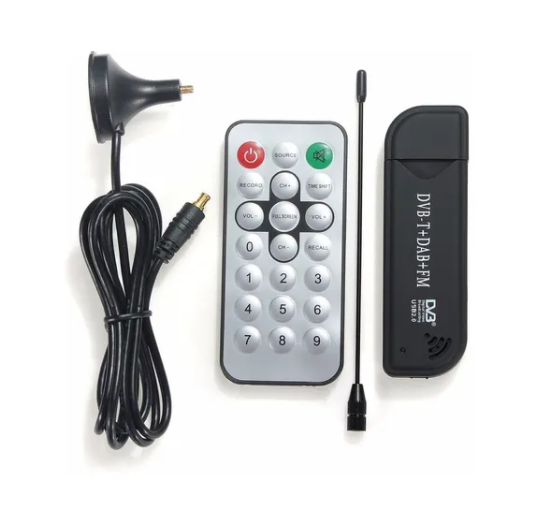
\includegraphics[scale=0.4]{images/sdr.png}
	\caption{Software Defined Radio utilizado para tomar las primeras mediciones}
	\label{SDR}
\end{figure}

En la figura \ref{llaves} podemos observar las primeras mediciones tomadas. Aquí distinguimos la estrategia de transmisión que se
utiliza. En un comienzo la señal posee un preámbulo, el cual es utilizado por el receptor para sincronizar el reloj del receptor  para 
decodificar correctamente los paquetes del transmisor. Después del preámbulo hay una palabra de sincronización que se utiliza para evitar 
choques con otros dispositivos que operan en esa banda y por último se encuentra la señal de código real.\par
Al presionar el botón del control remoto el preámbulo es enviado una única vez y luego se envía la palabra de sincronización y el
comando de acción repetidamente hasta que se deje de accionar. El espectro de la señal transmitida se puede observar en la figura \ref{espectro_ASK},
la cual es una simulación en el software AWR de una transmisión de datos random modulados ASK.

\begin{figure}[htb]
	\centering
	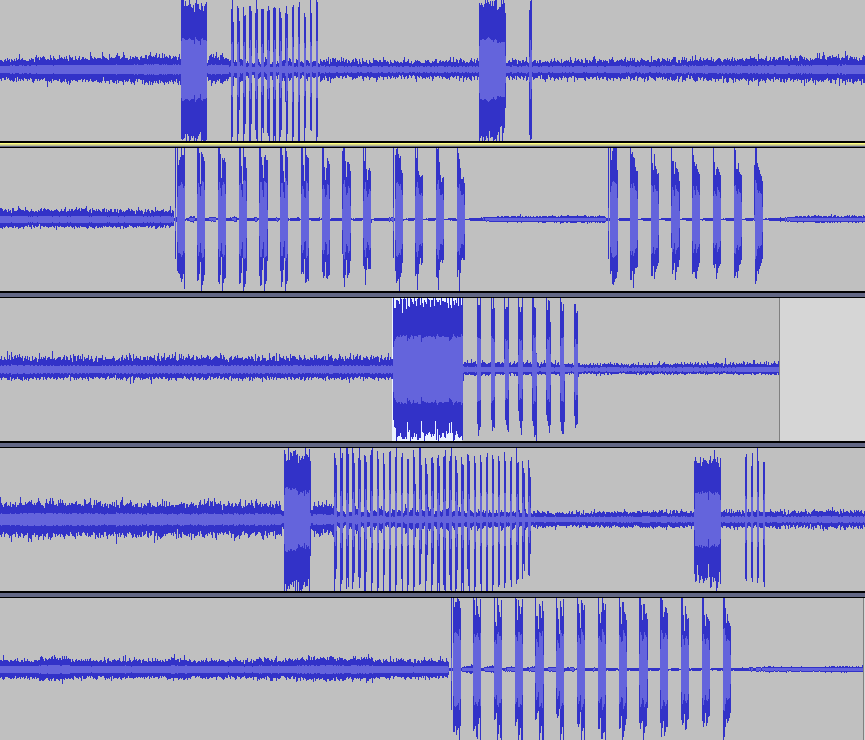
\includegraphics[scale=0.4]{images/llaves.png}
	\caption{Demodulación ASK de señales de controles remotos en 433,92 MHz}
	\label{llaves}
\end{figure}

\begin{figure}[htb]
	\centering
	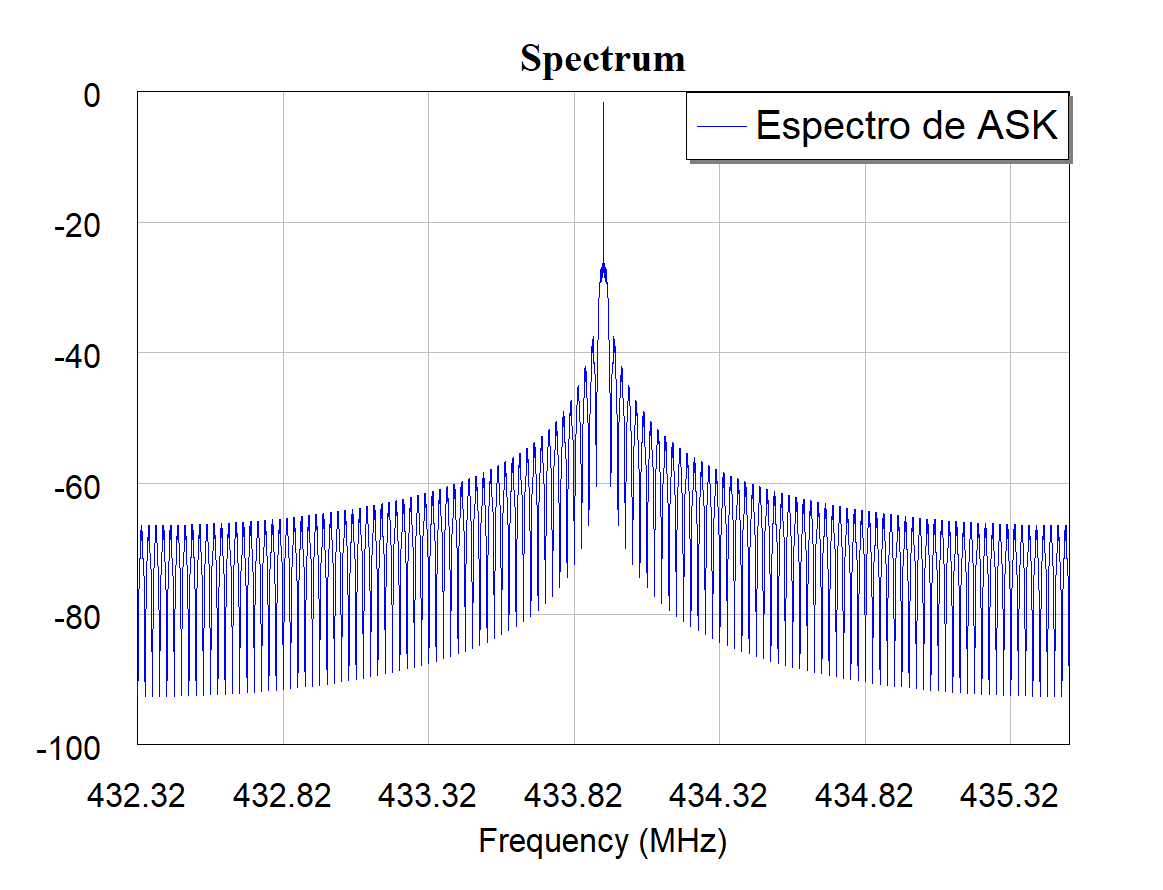
\includegraphics[scale=0.4]{images/espectro_ASK.png}
	\caption{Espectro de señal random bits modulada ASK en 433,92 MHz }
	\label{espectro_ASK}
\end{figure}

\subsection{Tipos de inhibiciones} \label{cap:tiposdeinhibiciones}

Un inhibidor, o en inglés jammer, es un dispositivo desarrollado con el objetivo de deteriorar la comunicación en un enlace de 
radiofrecuencia. Esto puede ser logrado mediante dos estrategias:

\begin{itemize}
    \item Inhibición por corrupción de datos
    \item Inhibición por saturación de etapa receptora

\end{itemize}

\subsubsection{Inhibición por corrupción de datos}

El ataque más evidente que se presenta para inhibir una comunicación es el de inyectar en el canal que se desea perjudicar una señal con 
datos aleatorios que perjudique la relación señal ruido (SNR) y dificulte la recepción para el sistema. \par
En el caso particular de los vehículos, los receptores de radiofrecuencia que se utilizan y sobre los que basamos nuestro análisis
son de 433,92 MHz con un filtro de ancho de banda de entrada de 300 KHz -como se analiza en [1].\par
El ancho de banda de recepción da lugar a sumar ruido en el canal, alterando así los datos recibidos por el demodulador. Una figura
ilustrativa se puede observa en la imagen \ref{fpb_jam} de [2].

\begin{figure}[htb]
	\centering
	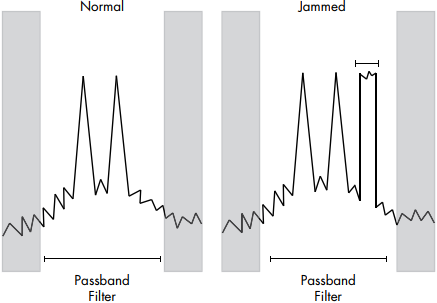
\includegraphics[scale=0.8]{images/fpb_jam.png}
	\caption{Presencia de inhibidor en ancho de banda de recepción}
	\label{fpb_jam}
\end{figure}

Existen diversas alternativas para efectivizar este tipo de interferencias. En la figura \ref{fpb_jam} se observa que se ha inyectado una
interferencia de ancho de banda angosto, pero también podría sumarse un tono, multitonos o sumar una señal de gran ancho de banda que 
tape completamente el canal. \par
Las alternativas antes mencionadas hacen referencia a inhibidores no inteligentes, los cuales están metiendo ruido constantemente. Hay otras 
alternativas de inhibiciones que de manera continua están escuchando el canal y cuando detectan una señal que 
desean interferir comienzan a emitir el ruido. Estos casos serán detallados más adelante.

\subsubsection{Inhibición por saturación de etapa receptora}

Los receptores de radiofrecuencia usualmente están diseñados asumiendo que se recibirá una pequeña señal de entrada, por lo que la primer
etapa presente es un amplificador de bajo ruido.  Este es clave para que el ruido del mezclador no afecte la relación señal ruido de las 
etapas siguientes. Entre las especificaciones importantes de dichos amplificadores de RF se incluyen la figura de ruido, la ganancia y la 
intercepción de intermodulación de tercer orden.\par
La influencia de grandes señales de interferencia se manifiesta de varias formas. Una de estas es en la intermodulación de tercer orden en la que dos señales, una pequeña (de interés) y la interferente (de gran amplitud), se superponen. La interferente podría saturar el receptor de modo que la señal de interés presente una pequeña ganancia como hace referencia [6] y [7]. Este efecto es causado por la no linealidad de tercer orden del sistema.

La saturación de un sistema suele tener un comportamiento de compresión  de la ganancia, decrementando la misma a medida de que la entrada aumenta.
Este efecto puede ser cualificado como el punto de 1 dB de compresión el cual está definido como el punto en el que la amplitud de la señal de 
entrada genera que la ganancia caiga 1 dB. Esto antes mencionado está claramente ilustrado en la figura \ref{eq:tercer_orden}.

\begin{equation}\label{eq:tercer_orden}
    y(t) \approx  a_1 x(t) + a_2 x^{2}(t) + a_3 x^{3}(t) 
\end{equation}

Donde \emph{y} es la salida del sistema y \(a_1, a_2, a_3 \) son coeficientes. Ahora supongamos que la entrada, como es de esperar con lo antes
descripto, resulta:

\begin{equation}\label{eq:entrada}
    x(t)=V_1 cos(\omega_1 t)+ V_2 cos(\omega_2 t)
\end{equation}

\(V_1\) representando a la señal de interés y \(V_2\) a la interferente.\par
Reemplazando en la ecuación \ref{eq:entrada} en \ref{eq:tercer_orden} y asumiendo que la interferencia es mucho más grande que la señal, 
la salida del sistema en la frecuencia de interés \(\omega_1\) resulta ser \ref{eq:intermodulacion}.

\begin{equation}\label{eq:intermodulacion}
    y(t) \approx \left( a_1 x(t) + \frac{3}{2} a_3 V_2^{2} \right) V_1  cos(\omega_1 t)
\end{equation}

Para que el sistema comprima la ganancia, como es evidente que sucede, el producto \(a_1 a_3 < 0\). De aquí se puede observar entonces que
la salida del sistema en la frecuencia deseada es función de \(V_2^{2}\), que la ganancia decae saturando el sistema y por ende se decrementa 
la SNR. Esto es fácilmente observable en la figura \ref{no_linealidad_e_tercer_orden}.

\begin{figure}[htb]
	\centering
	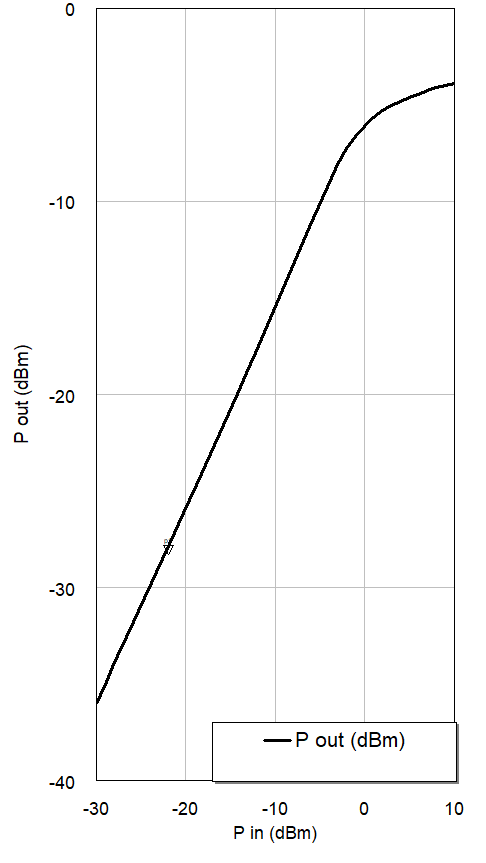
\includegraphics[scale=0.4]{images/no_linealidad_e_tercer_orden.png}
	\caption{Compresión de la ganancia}
	\label{no_linealidad_e_tercer_orden}
\end{figure}

\subsection{Estrategias de inhibición}

Antes hemos presentado los principios de inhibición que se pueden utilizar, en este apartado se tratará de una manera generalizada las diversas 
estrategias existentes para inhibir sistemas de comunicación. Cada una de estas tienen ventajas y desventajas, por lo que es necesario
hacer un análisis del ámbito de aplicación para elegir la más adecuada.


\subsubsection{Inhibición por ruido de banda ancha}

La característica principal de este tipo de estrategia es que introduce energía dentro de todo el ancho del espectro donde opera la comunicación.
Es aplicable a cualquier tipo de señal y es ideal para inhibir comunicaciones que tienen destinada una gran parte del espectro de frecuencias.\par
Este método tiene una fuerte desventaja y es que la potencia de interferencia aportada en el canal deseado tiene una muy baja densidad debido 
a es aplicada a un gran ancho de banda.

\subsubsection{Inhibición por ruido de banda parcial}

Este método opera inyectando ruido en bandas específicas del espectro, de modo que se efectúa la  inhibición en zonas de interés. Estas pueden ser continuas o discontinuas, por lo que se destina más inteligentemente la potencia consumida. El ejemplo más trivial aplicado a nuestro
campo sería el de un inhibidor que funcione en 433,92 y en 315 MHz, siendo  aplicable a todos los canales de comunicación de controles remotos.

\subsubsection{Inhibición por ruido de banda angosta}

Esta caso es el más utilizado en el campo de inhibición sobre el que nos centramos ya que permite puntualizar la potencia en una pequeña
banda aumentando la densidad de potencia espectral. Para su aplicación es necesario conocer precisamente el canal a atacar debido a que las 
comunicaciones inalámbricas de banda angosta poseen un angosto filtrado.

\subsubsection{Inhibición por tono}

Se utiliza una señal constante que se modula con la portadora resultando una señal de muy angosto ancho de banda. En sistemas de comunicación 
avanzados posee una alta eficiencia de interferencia ya que perjudica la recuperación de la sintonización a causa de que el receptor detecta 
la señal como una segunda portadora y de que más potencia por Hertz (densidad de potencia espectral) gracias a que está más concentrado
en el canal, como profundamente se analiza en [8].

\subsubsection{Inhibición por pulsos}

En esta estrategia nos enfocamos en el tiempo que se genera la interferencia. Se hace uso de uno de los métodos anteriores de inhibición
y se desata la misma de manera inteligente. De aquí surge el concepto de aplicar la estrategia a casos específicos, permitiendo, por ejemplo:
romper tramas específicas de datos conocidas cuando se detecta un CLT/RTS, interferir el dato de direccionamiento MAC o romper exclusivamente
la trama de datos.

\subsubsection{Inhibición por barrido y seguimiento}

Esta es una aplicación del ruido de banda parcial. Se realiza una variación rápida del posicionamiento espectral de la interferencia para inhibir
un gran ancho de banda teniendo un mejor aprovechamiento de la potencia disponible.\par
De esta alternativa se desprende la capacidad de seguimiento de la señal inhibidora, permitiendo contrarestar estrategias de comunicación que 
hacen uso de saltos de canales para ser efectivas.

\begin{figure}[htb]
	\centering
	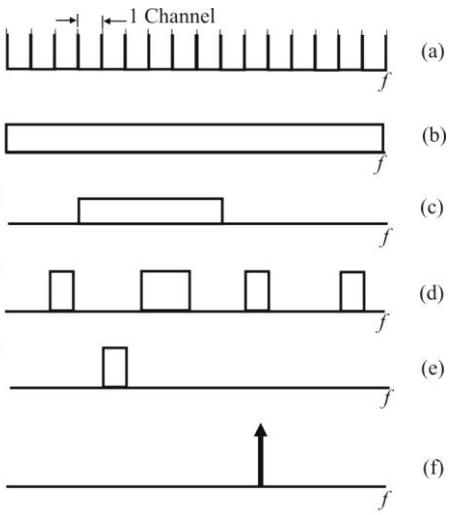
\includegraphics[scale=0.65]{images/tipos_de_jam.png}
    \caption{Donde a) es el canal a inhibir, b) inhibición por ruido de banda ancha, c) inhibición por ruido de banda parcial continuo, 
    d) inhibición por ruido de banda parcial discontinuo, e) inhibición por ruido de banda angosta, f) inhibición por tono }
	\label{tipos_de_jam}
\end{figure}

\subsubsection{Simulación de inhibición por ruido de banda parcial}

En este apartado se ha elegido la metodología de inyección de ruido de banda parcial para ser simulado y mostrar como decae la calidad de 
comunicación y, por ende, la capacidad de recepción de la información. La simulación fue realizada con el software AWR de Cadence.\par
El diagrama en bloques se puede observar en la figura \ref{bloques_inh}, este cuenta de 4 secciones principales:

\begin{itemize}
    \item Inhibidor de potencia variable: este bloque inyecta ruido blanco al sistema en la frecuencia definida como portadora, que en nuestro 
    caso es 433,92 MHz. La potencia de ruido va a variar entre 0 y -30 dBW, lo que sería igual a decir entre -30 y -60 dBm. 
    \item Emisor de señal: el emisor de señal es un modulador de ASK que modula una generación aleatoria de bits a 2500 baudios con la portadora.
    \item Medio de enlace: en este caso está representado con un combinador de señal RF, el cual va a servir para sumar la potencia de las dos
    señales anteriores.
    \item Demodulador: en esta instancia se produce la demodulación de la señal ASK más el ruido blanco agregado. Al final posee un bloque que
    se encarga de controlar el BER (Bit Error Rate), chequeando cuántos datos de los enviados efectivamente fueron recibidos. 

\end{itemize}

\begin{figure}[htb]
	\centering
	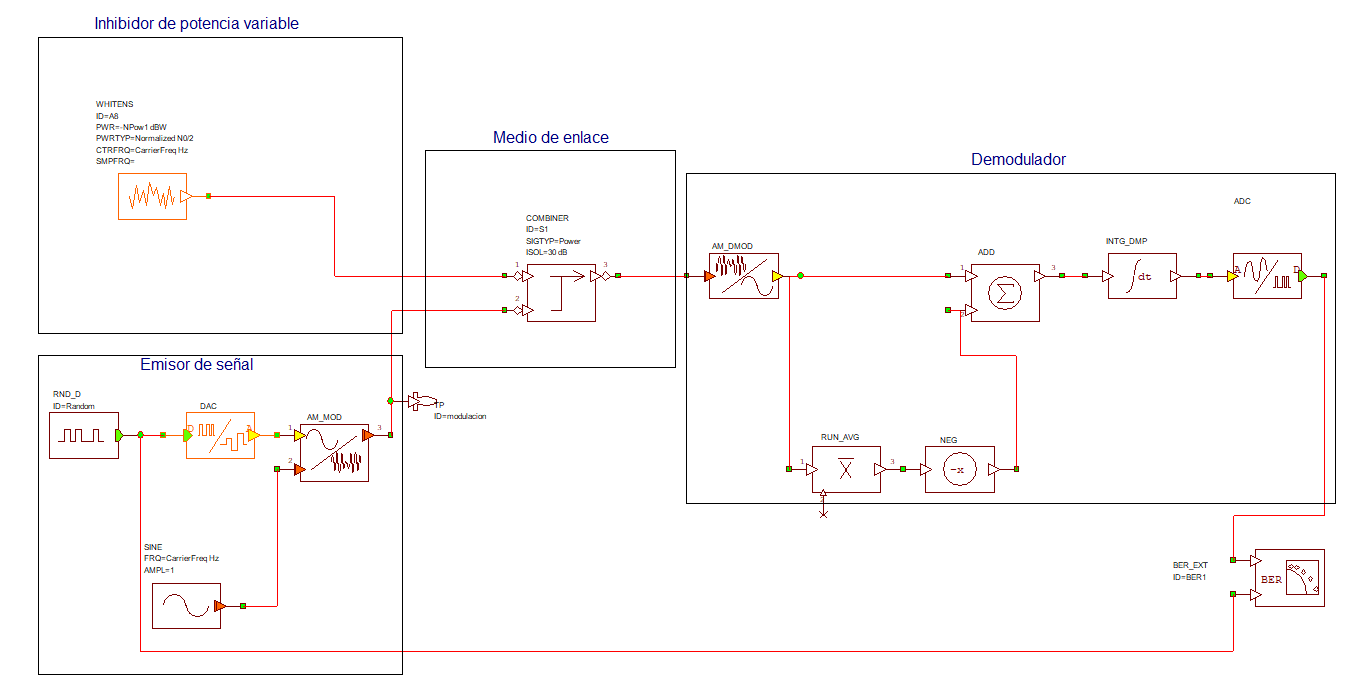
\includegraphics[scale=0.37]{images/bloques_inh.png}
    \caption{Diagrama en bloques de sistema de comunicación ASK inhibido}
	\label{bloques_inh}
\end{figure}

Como antes se menciona, y como se puede observar en la figura \ref{BER_ask}, el error de recepción alcanza su valor máximo cuando el ruido 
inyectado es de 0 dBW (-30 dBm). En la figura se puede leer un valor de BER = 0.4866, el cual es lógico debido a que la modulación ASK solo 
posee dos símbolos, por lo que la probabilidad de que coincida el dato generado por el ruido y el esperado es del 50\%. Por otro lado el valor
mínimo de error en la simulación propuesta sucede cuando la potencia del inhibidor es de -30 dBW (-60 dBm) teniendo un error de cuatro bits 
por cada diez mil recibidos.

\begin{figure}[htb]
	\centering
	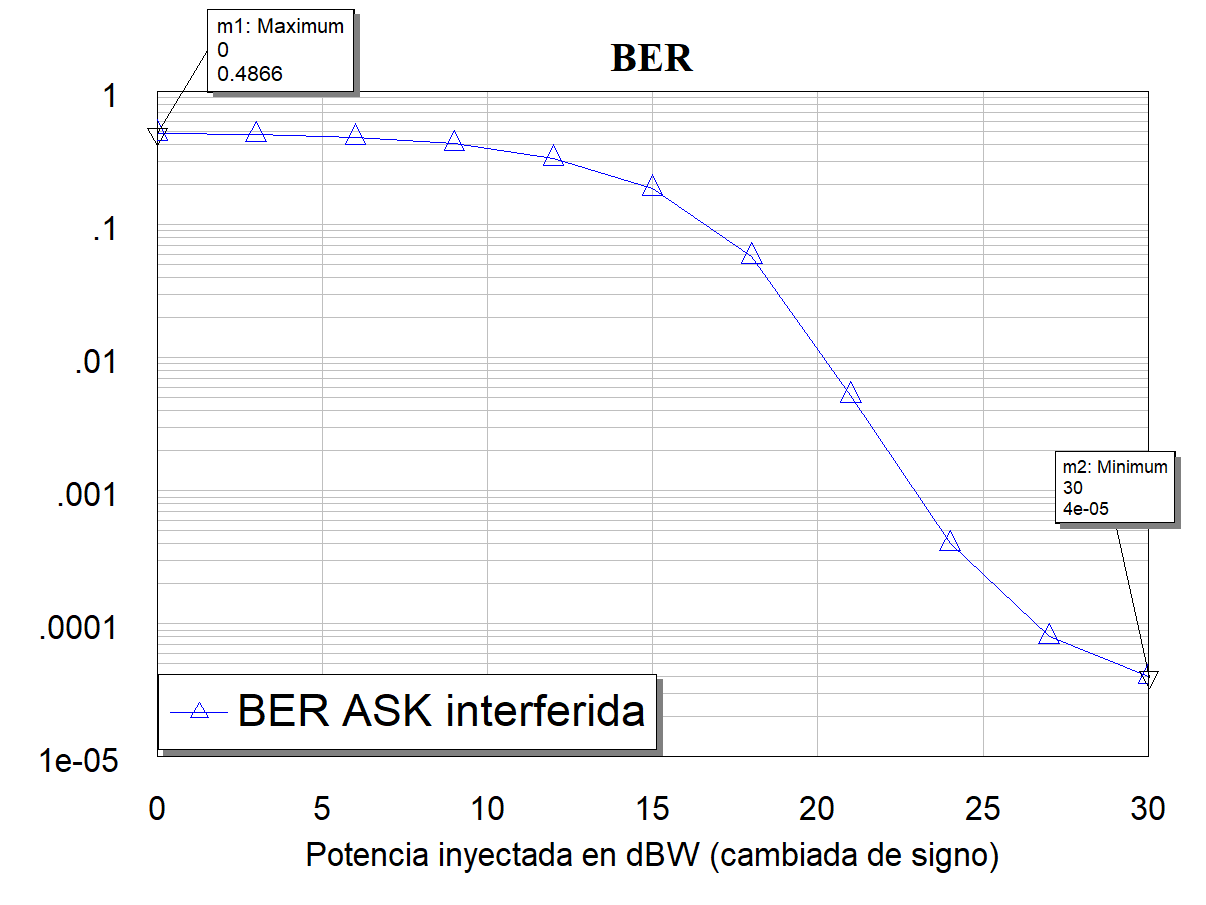
\includegraphics[scale=0.37]{images/BER_ask.png}
    \caption{Bit Error Rate para comunicación ASK inhibida.}
	\label{BER_ask}
\end{figure}

\subsection{Detección de inhibiciones}

En esta sección trataremos los métodos que pueden utilizarse para detectar interferencias en enlaces de radiofrecuencia. Es importante que 
sea robusta la detección, en principal que el funcionamiento del sistema que se pretende asegurar no pueda desatar una falsa alarma. En el caso
puntual de aplicación de este proyecto, el sistema debería poder identificar una inhibición y no identificar como tal a las señales de controles 
remotos que van a estar funcionando en el área circundante. 
Hay algunas características las cuales son naturales pensar como sensibles de analizar para detectar inhibiciones, y estas son: 

\begin{itemize}
    \item Potencia de la señal recibida
    \item Sensado temporal de portadora
    \item Ocupación del canal

\end{itemize}

\subsubsection{Potencia de la señal recibida}

Como antes se ha definido, el receptor sufre compresión de ganancia en su primera etapa amplificadora cuando la potencia recibida es alta
comparado a la potencia de señal que se espera recibir y para el que fue diseñado. Es por esto que resulta natural analizar los niveles de
potencia recibidos, estableciendo un valor a partir del cual se señale como alarmante para la correcta recepción de la información. 
En el caso particular de los dispositivos de control remoto en los sistemas de seguridad vehicular resulta más sencillo el análisis 
debido a que los dispositivos emisores que se utilizan son de baja potencia comparado a la necesaria para saturar un receptor típico.\par
En [7] se realiza el análisis del receptor MAX1470 [1], muy difundido en sistemas de control remoto tanto en el ámbito automotriz como también
en sistemas de portones de apertura inalámbrica, sistemas de seguridad, sensores inalámbricos y mucho más. Este integrado es un receptor de 
ASK superheterodíneo de bajo costo que posee un mezclador de rechazo de imagen que mezcla la señal a una frecuencia intermedia de 10,7 MHz. En
la figura \ref{compresion_max} se puede observar que la ganancia del sistema de recepción se aplana aproximadamente con una entrada de -35 dBm.

\begin{figure}[htb]
	\centering
	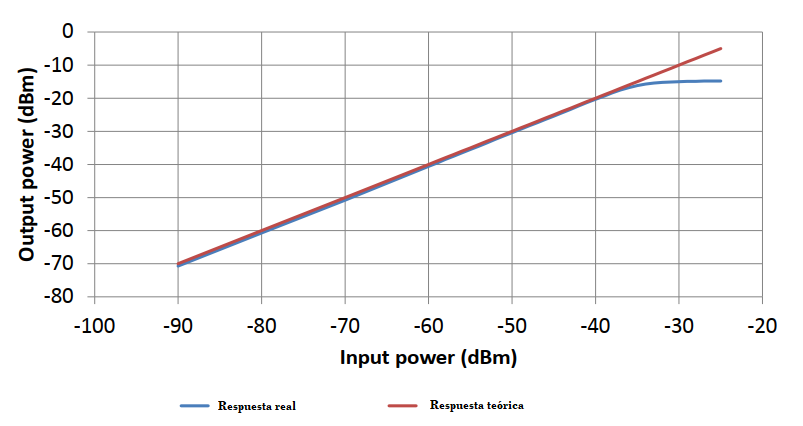
\includegraphics[scale=0.5]{images/compresion_max.png}
    \caption{Curva de ganancia de MAX1470}
	\label{compresion_max}
\end{figure}


\subsubsection{Sensado temporal de portadora}

Esta es una estrategia muy utilizada en sistemas de comunicación en que se realiza un envío efectivo de paquetes cuando se detecta que el canal 
de transmisión está desocupado. Esta característica hace sensible al sistema de ser engañado dejando presente una señal portadora de información
que engañe a los dispositivos emisores de la red.\par
En nuestro caso no nos detendremos a hacer un análisis profundo de esta metodología ya que es ajena a nuestro potencial mecanismo de detección
debido a que, como se menciona en 3.1.2, el control remoto emite señal cuando es accionado un botón que este posee, haciéndolo de manera continua
hasta que deje de ser apretado. Es fácil ver que esta característica de la comunicación hace inútil aplicar esta estrategia de detección

\subsubsection{Ocupación del canal}

El sistema de comunicación que nos basamos para desarrollar este trabajo tiene la particularidad de que la comunicación unilateral que sucede
entre los dispositivos de emisión (controles remotos) y recepción (vehículos) tienen una muy baja tasa de ocupación de canal. Esto se debe a 
la trama de datos empleada. La misma, como antes fue explicado, posee un período de sincronización que es una rápida variación de estados, para
que el receptor pueda engancharse en fase a la recepción, y luego envío de paquetes de datos separados por espacios vacíos de información. Esta
característica nos da una relación de bits en alto recibidos respecto a los medidos de un valor porcentual muy bajo. Es por esto que esta medición
en el canal, usandola estratégicamente, nos puede dar mucha información de lo que está sucediendo.
 % Introduccion - Corregido
\pagebreak

\chapter{Características generales del diseño}
\section{Objetivos globales del sistema}

En base a la información recolectada establecemos los requerimientos base del que se parte para el diseño del producto final. Creemos adecuado
realizar la separación de requerimientos en primarios y secundarios, ya que el sistema a desarrollar está enmarcado en el proyecto final de la 
carrera de grado de ingeniería electrónica donde, en conjunto con la cátedra, se intenta que los proyectos puedan culminarse en un plazo de 
tiempo lógico para la obtención del título, dando la posibilidad de seguir explayándose en el mismo a posterior. \par

De este modo, como objetivos primarios se establecen:

\begin{itemize}
    \item Identificar la presencia de señales con una potencia suficiente para inhibir la comunicación: como en el marco teórico se ha 
    estudiado en profundidad, la etapa amplificadora receptora sufre una compresión de la ganancia cuando en su entrada hay presente 
    una señal de alto nivel de potencia. Es por esto que se establece como requerimiento del sistema poder identificar una señal que cumpla con
    estas características.
    \item Medir la ocupación del canal: Ha quedado claro que la trama de comunicación de las llaves remotas con los receptores de los automóviles 
    poseen características de espaciado entre paquetes de datos transmitidos, es por esto que el sensado de la ocupación del canal se vuelve 
    una medida crucial para determinar si hay o no presencia de interferencias.
    \item Activar alarmas sonoras y visuales en caso de estar en presencia de una inhibición: el sistema debe tener la capacidad de determinar 
    si hay presente una inhibición en su área de operación y, de ser así, debe disponer de métodos para dar alerta local de lo que está sucediendo.
    \item Disponer de comunicación a sistemas externos complementarios: un requisito del sistema es que posea la capacidad de enviar la información recolectada
    a un lugar remoto. Se prefiere la utilización de una metodología de comunicación inalámbrica y ampliamente distribuida.
    \item Cargar los datos en una base de datos: es importante que la información de las inhibiciones detectadas sea subida a una base de datos
    que permita visualizar de manera remota y en tiempo real lo que está sucediendo con los sistemas de seguridad activos, brindando la posibilidad 
    de generar estadísticas y observar qué tipos de inhibidores están operando en la zona.
    \item Orientar el diseño del proyecto a la optimización de costos y recursos: es muy importante para el curso del trabajo que el diseño 
    se realice haciendo uso racional de los recursos disponibles, apuntando a la posibilidad de producir muchas unidades del sistema de seguridad
    y obtener ganancias.

\end{itemize}

Como objetivo secundario se define:

\begin{itemize}
    \item Estimar la procedencia de la interferencia: el único objetivo secundario del sistema es que tenga la capacidad, mediante el método 
    más conveniente, de determinar la posición estimada de la fuente de interferencia activa. Esto está planteado de esta manera debido a que 
    se desconoce la factibilidad de su realización en el marco del proyecto de fin de grado de ingeniería electrónica.
\end{itemize}

\section{Esquema de funcionamiento}

En la figura \ref{bloques_funcionamiento} se puede observar el sistema planteado para solucionar el desafío de detectar inhibiciones en los sistemas
de seguridad vehicular. El mismo contará con nodos detectores que operarán en 433,92 MHz, un canal de comunicación hacia la central, haciendo
uso de un protocolo que más adelante se detallará y una central de operación donde se decidirá si hay o no inhibición en su área de operación
desatando las alarmas pertinentes y subiendo la información al servidor. \par

\begin{figure}[htb]
	\centering
	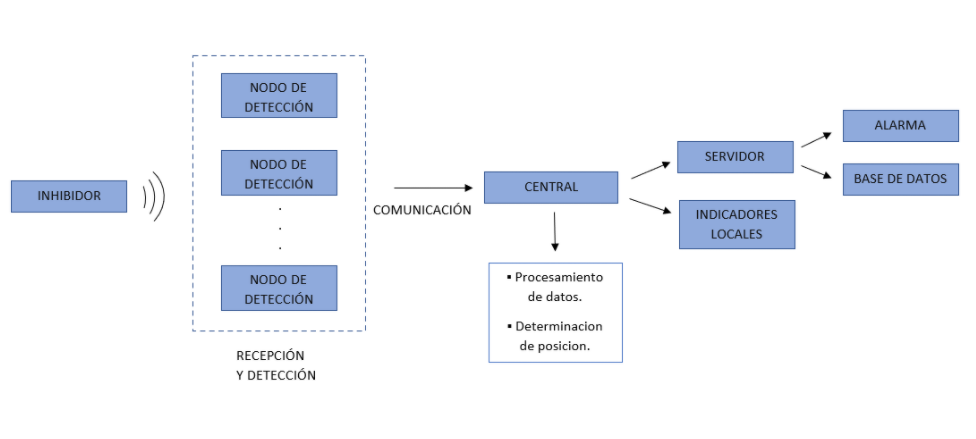
\includegraphics[scale=0.53]{images/bloques_funcionamiento.png}
    \caption{Diagrama en bloques sobre el funcionamiento del sistema global}
	\label{bloques_funcionamiento}
\end{figure}

\section{Subsistemas que lo componen}

En esta sección únicamente se hará mención de los subsistemas que componen al producto final, más adelante se detallará en capítulos el funcionamiento 
particular de cada uno de estos bloques.

\begin{itemize}
    \item Nodo receptor 
    \begin{itemize}
          \item Microcontrolador STM32F103C8T6.
          \item Receptor de RF. 
          \item Integrado para comunicación RS-485.
    \end{itemize}
    \item Central de procesamiento 
    \begin{itemize}
          \item Microcontrolador STM32F103C8T6.
          \item Integrado para comunicación GSM/GPRS. 
          \item Integrado para comunicación RS-485.
    \end{itemize}
    
\end{itemize}
 % Características generales del diseño - Corregido
\pagebreak


\chapter{Selección de componentes}
En este capítulo se procede a exponer las características mas importantes  de los componentes del sistema, así como las consideraciones y 
posibilidades que tuvimos en cuenta en el proceso de selección de los mismos. \par

En el momento de comenzar este proyecto, rápidamente nos vimos ante la necesidad de seleccionar los componentes de nuestro sistema. 
En este proceso tuvimos en cuenta los objetivos y el diagrama de funcionamiento general que se trató en el capítulo de características que precede,
además de otras consideraciones como el costo, los conocimientos previos del equipo sobre el componente, disponibilidad, etc. 
Para poder explicar como fue este proceso, dividimos el sistema en tres etapas: Recepción, procesamiento, y comunicación.

\section{Etapa receptora de RF} \par
De acuerdo al planteamiento del sistema, una parte crucial en el funcionamiento del mismo es la recepción de la señal de interés.
Vale recordar que la etapa de recepción se encuentra presente en todos los nodos del sistema, por lo que las diferencias de costos
en este apartado se ven multiplicadas.\par
La recepción debe cumplir con las siguientes características:

\begin{itemize}
    \item Antena para 433MHz. Es el primer componente a tener en cuenta cuando hablamos de comunicaciones inalámbricas. En este caso, 
    este transductor nos servirá para obtener la energía eléctrica que podemos entender y analizar, a partir de la ondas electromagnéticas
    emitidas por la llave de automóvil y por los inhibidores. Planteamos la posibilidad de utilizar dos tipos de antenas, del tipo 
    omnidireccional o una con la capacidad de generar un barrido, característica importante si se quiere obtener la posición del inhibidor.

    \item Demodulación de señales ASK en 433MHz. Es el principal requerimiento de la recepción debido a las características de las 
    comunicaciones presentes en los sistemas de seguridad de vehículos.

    \item Medición de RSSI. La medición del nivel de potencia de la señal recibida es crucial para poder identificar adecuadamente
    a los inhibidores. También cumple un rol indispensable en uno de los objetivos secundarios mas desafiantes del sistema como lo es la obtención
    de la posición del elemento inhibidor mediante triangulación.

    \item Comunicación con microcontrolador. Es importante tener en cuenta las posibilidades que nos ofrece esta etapa a la hora de comunicarse
    con la siguiente. Los datos obtenidos de la recepción de la señal serán procesados por un microcontrolador.

\end{itemize}

Luego de estudiar las mejores opciones llegamos a una que consiste en utilizar un esquema como el que vemos en la figura
\ref{EtapaReceptora1}. En primer lugar elegimos utilizar una antena omnidireccional, es la opción que nos permite reducir los precios
y simplificar el proyecto al evitar sistemas de matrices antenas o antenas con rotación.
El inconveniente de esta elección, es que la antena omnidireccional no nos entrega información referida al ángulo en que recibe la señal, por lo que
complica la obtención de la posición. Sin embargo, todavía es posible comparando la lectura del nivel de RSSI de cada nodo.
Luego encontramos un divisor de potencia de RF que se encarga de entregar la señal al demodulador ASK, y al medidor de potencia. \par

\begin{figure}[htb]
	\centering
	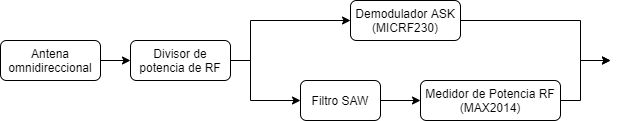
\includegraphics[scale=0.6]{images/Opcion1.png}
    \caption{Etapa receptora - primer opción}
	\label{EtapaReceptora1}
\end{figure}


Vemos que este diagrama cumple con las características anteriormente expuestas. Sin embargo, al final nos decantamos por otra opción, 
que consiste en utilizar el circuito integrado CC1101 (transceptor de RF hasta 1GHz). La incorporación de este nos permite reducir mucho los costos y simplificar
el sistema sin sacrificar características importantes. \par
En la figura \ref{EtapaReceptora2} vemos como resulta el nuevo diagrama de la etapa receptora. \par

\begin{figure}[htb]
	\centering
	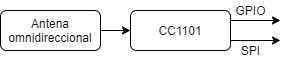
\includegraphics[scale=0.6]{images/Opcion2.png}
    \caption{Etapa receptora - opción elegida}
	\label{EtapaReceptora2}
\end{figure}

A simple vista podemos apreciar que se reducen la cantidad de componentes. Esto se debe a que el módulo CC1101 es capaz de demodular la señal y
entregar la secuencia de bits mediante un pin de GPIO, así como también medir la potencia de la señal y comunicar el valor mediante comunicación SPI.
La única desventaja de esta opción es que posee peor rango de RSSI que un componente medidor de potencia específico para ese fin,
esto provoca que señales de gran potencia saturen nuestro receptor y nos imposibilite triangular de manera correcta, sin embargo la determinación 
de la posición es un objetivo secundario. \par
En la sección \ref{cap:cc1101} se exponen en detalle las características del módulo.\par

\subsection{CC1101} \label{cap:cc1101}
\subsubsection{Transceptor}
\paragraph{Descripción del componente} \par


\begin{figure}[htb]
	\centering
	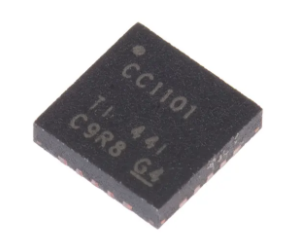
\includegraphics[scale=0.6]{images/CC1101.png}
    \caption{Transceptor CC1101}
	\label{fig:cc1101}
\end{figure}

El integrado CC1101 es un transceptor de frecuencias inferiores a 1GHz de bajo costo para aplicaciones inalámbricas de baja potencia. Está destinado principalmente
a aplicaciones ISM (industrial, científico y médico) y bandas de frecuencia SRD (Dispositivo de corto alcance) a 315, 433, 868 y 915Mhz, pero puedo ser programado 
para funcionar en otras bandas. El transceptor RF está integrado con un módem de banda base configurable que admite varios formatos de modulación.\par 
Proporciona un amplio soporte de hardware para manejo de paquetes, almacenamiento en búffer de datos, transmisiones de ráfagas, evaluación de canal,
indicación de calidad de enlace y wake-on-radio. \par 
En un típico sistema, el CC1101 se utiliza junto con un microcontrolador y algunos componentes pasivos adicionales.

\paragraph{Características generales} \par

En este apartado mostramos algunas características importantes del CC1101 sin extendernos demasiado. Si se quiere mas información sobre este integrado ver \ref{bib:cc1101}.

\begin{itemize}
    \item Alimentación de 3.3V
    \item Sensibilidad: 
    \subitem -116 dBm a 0.6kBaud en 433MHz
    \subitem -112 dBm a 1.2kBaud en 868 MHz
    \item Velocidad de datos: Hasta 250kbaud en ASK.
    \item Bajo consumo de corriente: 14.7mA en RX.
    \item Admite 2-FSK, 4-FSK, GFSK y MSK, así como OOK y ASK.
    \item Medición de RSSI entre -110dBm a -20dBm.
    \item Interfaz SPI, a través de la cual se puede configurar todos los registros.
    \item Filtro digital de banda ancha programable. 58-812kHz.
\end{itemize}

\subsubsection{Módulo}

El modulo aporta simplicidad al sistema, ya que contiene los componentes pasivos necesarios para el funcionamiento del CC1101. También permite mejor acceso a los pines 
del integrado y tiene conexión SMA para antena. En nuestro caso particular, este módulo fue necesario debido a que simplifica la soldadura manual y porque
tiene una gran disponibilidad en el mercado.

En la figura \ref{fig:sch_cc1101} podemos ver el esquemático del módulo y en la figura \ref{fig:module_cc1101} podemos ver su aspecto físico.

\begin{figure}[htb]
	\centering
	\includegraphics[scale=0.6]{images/EsquemáticoCC1101.jpg}
    \caption{Esquemático CC1101}
	\label{fig:sch_cc1101}
\end{figure}

Se puede observar en el esquemático, que el módulo es muy simple en cuanto a los componentes que posee. Pero aún así es muy útil para nuestra aplicación.

\begin{figure}[htb]
	\centering
	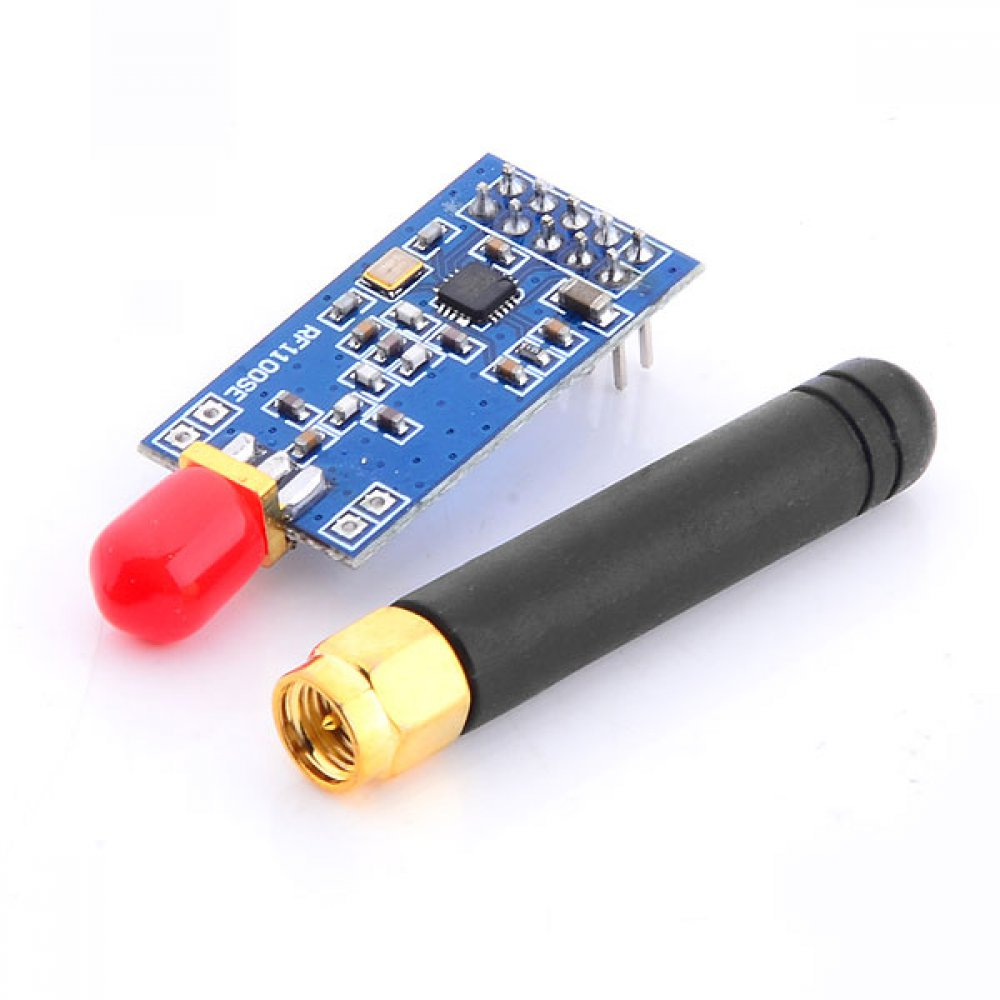
\includegraphics[scale=0.2]{images/modulo_cc1101.jpg}
    \caption{Módulo CC1101}
	\label{fig:module_cc1101}
\end{figure}

\section{Comunicación}

La comunicación se puede dividir en dos partes, la primera referida a la comunicación entre los nodos y la central y la otra, referida a la comunicación
de la central con un servidor web.


\subsection{Comunicación local}

Según nuestros objetivos, la comunicación debe reunir las siguientes características:

\begin{itemize}
    \item Resistencia a ataques de inhibidores. Es importante que la comunicación local no sea vulnerable a los mismos ataques que intentamos identificar, ya que
    si fallara la comunicación entre los nodos y la central el sistema no puede dar aviso de la presencia de una señal interferente.
    \item Comunicación bidireccional. Para establecer una red multinodal adecuada necesitamos un sistema de comunicación half-duplex o full-duplex, ya que 
    la central comandará a los nodos, los cuales le responden con la información que la central les requiere.
    \item Distancia mayor a 1000m. Es probable que el sistema sea instalado en lugares abiertos como estacionamientos, por lo que necesitamos un protocolo de 
    comunicación capaz de funcionar a largas distancias.
    \item Buena velocidad de comunicación. No requerimos de velocidades muy altas, sin embargo es una característica a tener en cuenta.
    \item Cableado de bajo costo. Como ya mencionamos, es probable que la distancia entre nodos sea grande, por lo que el precio del cableado debe ajustarse 
    a nuestros objetivos.

\end{itemize}

Teniendo en cuenta las necesidades y analizando las opciones, determinamos que la mejor opción para nuestra aplicación es usar el estándar de comunicación RS485. 
Este está definido como un sistema de bus diferencial multipunto, ideal para transmitir a altas velocidades sobre largas distancias y a través de canales ruidosos.
El medio físico de transmisión es un par trenzado con una longitud máxima de 1200 metros operando entre 300 y 19200 bit/s y la comunicación semiduplex.\par
Las especificaciones de este estándar son:

\begin{itemize}
    \item Interfaz diferencial
    \item Conexión multipunto
    \item Alimentación de 5V
    \item Hasta 32 estaciones 
    \item Velocidad Máxima de 10Mbit/s (a 12 metros)
    \item Longitud máxima de alcance de 1200 metro (a 100kbit/s)
    \item Rango de bus de -7V a +12V

\end{itemize}

Para nuestra aplicación usaremos el RS485 en combinación de la UART de nuestro microcontrolador, por lo que necesitaremos utilizar un transceptor MAX485 
(ver sección \ref{cap:max485}). Se dispone uno en cada nodo y en la central. El MAX485 tiene la capacidad de transformar los datos de la UART al estándar
RS485 y viceversa. \par

\subsection{MAX485} \label{cap:max485}

MAX 485 es un transceptor de baja potencia para comunicación RS-485 y RS-422. Cada integrado contiene un controlador y un receptor.\par 
La velocidad de respuesta del controlador del MAX485 no está limitada, lo que les permite transmitir hasta 2,5 Mbps. Estos transceptores
consumen entre 120 µA y 500 µA de corriente de suministro cuando están descargados o completamente cargados con controladores desactivados.
Todas las piezas funcionan con un solo suministro de 5V. 

\begin{figure}[htb]
	\centering
	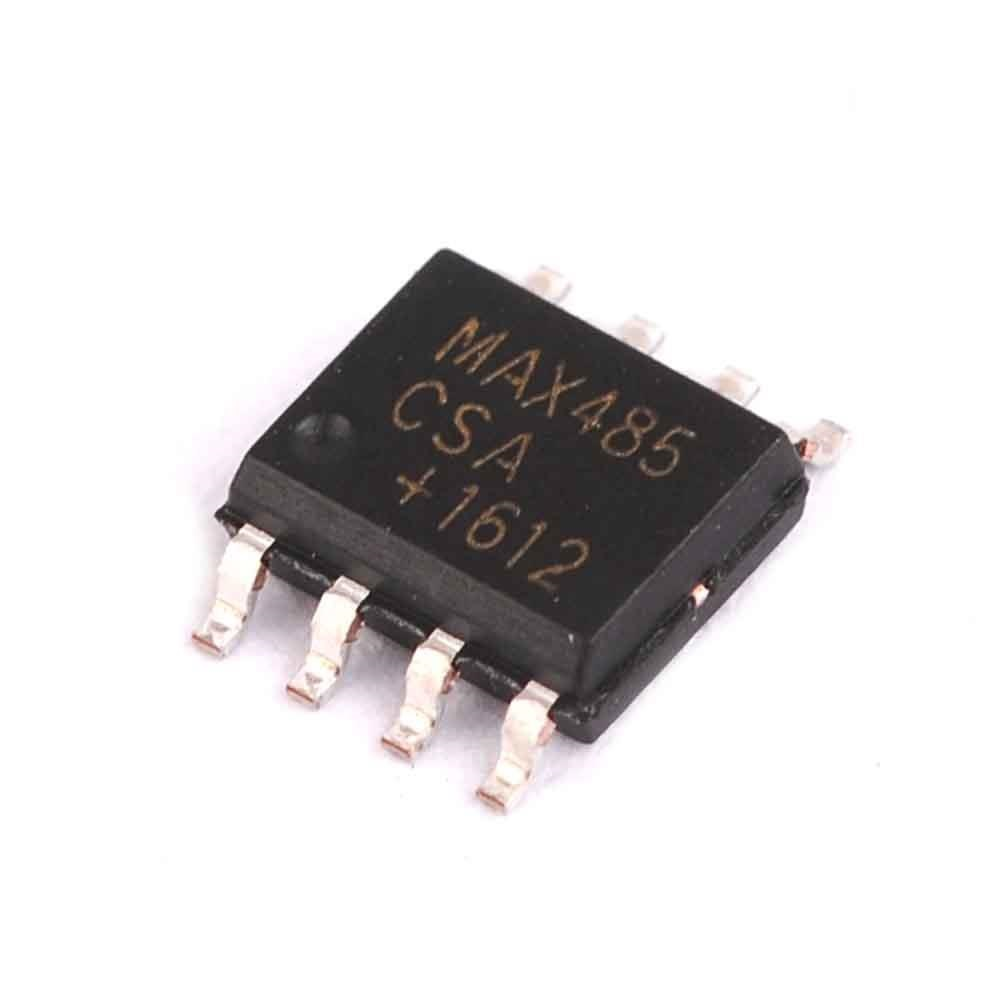
\includegraphics[scale=0.5]{images/max485.jpg}
    \caption{Max 485}
	\label{fig:max485}
\end{figure}

Los controladores tienen limitación de corriente de cortocircuito y están protegidos
contra una disipación de energía excesiva mediante un circuito de apagado térmico que coloca las salidas del controlador en un estado de alta 
impedancia. La entrada del receptor tiene una característica a prueba de fallas que garantiza una salida lógica alta si la entrada está en 
circuito abierto. El MAX485 está diseñado para aplicaciones semidúplex.


\subsection{Comunicación con Servidor Web}

Una de las características mas importantes del proyecto, es la capacidad de subir la información a un Servidor Web, por lo que es indispensable que la central disponga
de conexión a internet.\par
Debido a que no podemos asegurar que en el lugar donde se instale el sistema cuente con conexión a internet cableada o WiFi, decidimos utilizar conexión GPRS/2G. \par
En el mercado podemos encontrar varios módulos para este tipo de conexiones. En la tabla \ref{tab:gsm} podemos ver algunas opciones.

\begin{table}[t]
    \begin{center}
        \begin{tabular}{ | m{3cm} | m{3cm} | m{3cm} | m{3cm} | }
        \hline Módulo & SIM800L & SIM900 & A6  \\ \hline
        Velocidad de transmisión & 1200 bp - 115200 bp. & 1200bp - 115200bp. & 1200bp - 115200bp. \\ \hline
        Tensión de operación & 3.4V - 4.4V & 9V - 20V & 3.3V - 4.2V \\ \hline
        Corriente & Hasta 2A & Hasta 2A & Hasta 2A\\ \hline
        Comunicación & Comunicación serial & Comunicación UART & Comunicación serial\\ \hline
        Precio & 13,39 usd &  48,70 usd & 18,26 usd\\ \hline
        
        \end{tabular}
        \caption{Módulos GSM/GPRS disponibles en el mercado}
        \label{tab:gsm}   
    \end{center}
\end{table}

Nosotros elegimos el módulo sim800l por dos razones, la primera es el bajo precio comparado con el sim900 y la segunda por la experiencia previa
que disponíamos con este módulo.
En la sección \ref{cap:sim800l} se detallan las características de este componente.


\subsection{SIM800L} \label{cap:sim800l}

\subsubsection{Descripción del componente}

Utilizamos el SIM800L a través de un módulo del mismo nombre, como se suele utilizar normalmente. El módulo nos permite acceder a los pines 
mas importantes del SIM800L para manejarlo desde un microcontrolador.\par
Consiste en un circuito integrado cuatribanda que permite agregar funcionalidades avanzadas de comunicación a través de la red celular, como mandar mensajes de texto,
datos o realizar llamadas en un tamaño sumamente compacto. 

\begin{figure}[htb]
	\centering
	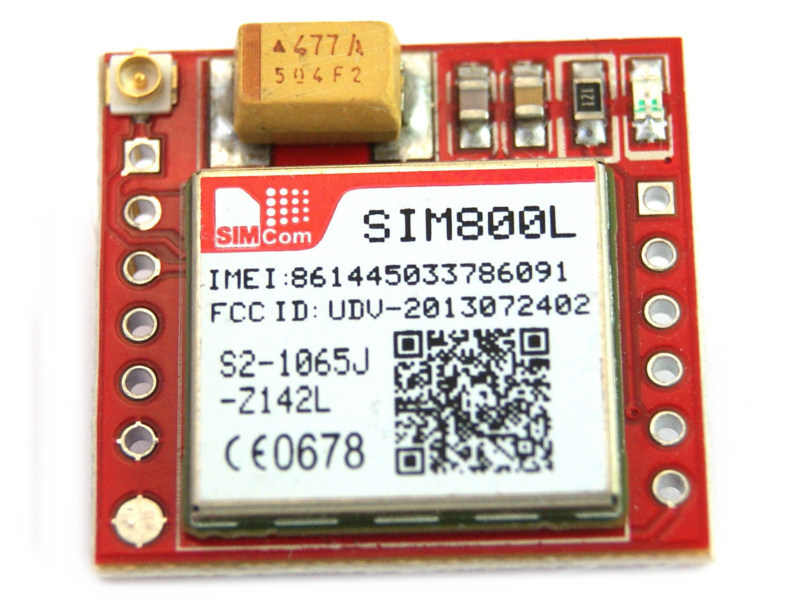
\includegraphics[scale=0.2]{images/sim800l.png}
    \caption{Módulo SIM800L}
	\label{fig:sim800l}
\end{figure}

\subsubsection{Características Generales}

A continuación se listan algunas características importantes de este módulo. Sin embargo, si se quiere ver en mayor profundidad ver \ref{bib:sim800}.

\begin{itemize}
    \item Tensión de operación: 3.4V - 4.4V
    \item Nivel lógico de 3-5V
    \item Consumo de corriente:
    \subitem Máximo: 500mA con picos de 2A
    \subitem En reposo: 0,7mA
    \item Interfaz serial UART
    \item Quad-Band 850/900/1800/1900MHz. Conexión a cualquier red mundial por 2G.
    \item Controlado por comandos AT
    \item Velocidades de transmisión serial desde 1200bps hasta 115 200 bps
    \item Tamaño de la SIM: Micro SIM
\end{itemize}

\section{Procesamiento} \par

Tanto en los nodos como en la central, es indispensable el uso de un microcontrolador. En el caso del nodo, se encarga de comunicarse con la etapa receptora,
procesar la información y decidir si la señal recibida proviene de un inhibidor, luego debe ser capaz de comunicarse con el MAX485 para establecer la comunicación
RS485 con el resto del sistema. En la central, el microcontrolador es el encargado de recibir la información de nodos a través del MAX485 y,
en caso de la presencia de una inhibición, activar las alarmas correspondientes y actualizar la información en el servidor web mediante el módulo sim800l. \par

El microcontrolador que utilizamos, tanto para los nodos como en la central, es el STM32F103C8T6. La decisión de utilizar este se tomó debido 
a sus características, el bajo precio y sobre todo porque ya contábamos con experiencia en su uso.
En este caso, decidimos utilizar un módulo de desarrollo llamado "Blue Pill". Las características de esta placa la podemos ver en la sección \ref{cap:stm32}.

En la tabla \ref{tab:uC} podemos ver una comparación entre nuestro microcontrolador y otras opciones similares de otros marcas.

\begin{table}[t]
    \begin{center}
        \begin{tabular}{ | m{3cm} | m{3cm} | m{3cm} | m{3cm} | }
        \hline  & Blue Pill & Arduino Nano & PIC18F4520  \\ \hline
        Procesador & ARM 32 bits & AVG 8bits & PIC 8bits \\ \hline
        Frecuencia de Funcionamiento & 72MHz &20MHz & 8MHz \\ \hline
        Memoria FLASH & 64 o 128kb & 32kb & 32kb\\ \hline
        SRAM & 20Kb & 2Kb & 2Kb \\ \hline
        comunicación & USB. SPI. I2C. USARTs &  USB. SPI. I2C. USARTs & EUSART. SPP. USB. SPI. I2C\\ \hline
        Precio & 6,20 usd &  6,67 usd & 13,39 usd\\ \hline
        
        \end{tabular}
        \caption{Comparación de microcontroladores}
        \label{tab:uC}   
    \end{center}
\end{table}

Es importante añadir que podemos programar la Blue Pill mediante un programador STLINK v2, que tiene un precio bajo comparado a otros programadores, y
utilizar el programa STM32CubeIDE del fabricante para debuggear el sistema, característica que fue muy importante en el desarrollo del proyecto.\par
En la sección \ref{cap:stm32} ahondamos mas sobre este módulo y el microcontrolador en cuestión. 

\subsection{Blue Pill STM32} \label{cap:stm32}
\subsubsection{STM32F103C8T6}

Es un microcontrolador perteneciente a la linea de rendimiento medio de la familia STM. Incorpora el núcleo RISC ARM Cortex de 32 bits de alto rendimiento,
posee memorias integradas de alta velocidad y una amplia gama de entradas y salidas. Este dispositivo ofrece dos ADC de 12bits, tres temporizadores de 16bits
de uso general mas un temporizador PWM, así como diversas interfaces de comunicación.\par 
Es apto para gran variedad de aplicaciones, como unidades de motor, control de aplicaciones, equipos médicos y portátiles, periféricos
de PC y juegos, plataformas GPS, aplicaciones industriales, PLC, inversores, impresoras, escáneres , sistemas de alarma, videoporteros y HVAC.

A continuación se listan algunas de las características que nos parecen mas importantes:

\begin{itemize}
    \item Tensión de operación: 2 a 3,6V
    \item Frecuencia de 72MHz
    \item Memorias integradas de alta velocidad
    \subitem Memoria Flash de 128Kbytes
    \subitem Memoria SRAM de hasta 20Kbytes
    \item Interfaces de comunicación: Dos I2C y SPI, tres USART y un USB.
    \item 37 GPIOs
    \item Dos ADC de 10 canales.
\end{itemize}

\subsubsection{Módulo Blue Pill}

En nuestro sistema utilizamos la placa de desarrollo llamaba Blue Pill. Esta placa incorpora al STM32F103C8T6 y aporta los componentes pasivos
adecuados para su uso, además de dos cristales, entrada microUSB, leds indicadores, botón de reset e integrado para regulación de tensión. \par
Incorporar esta placa simplifica el diseño de nuestros PCB, ya que nos facilita el acceso a los pines del microcontrolador y posibilita la conexión
con el programador, además nos permite desarrollar un proyecto donde soldemos de forma manual los componentes, reduciendo costos.\par
En la figura \ref{fig:sch_bluepill} vemos el esquemático de esta placa.

\begin{figure}[htb]
	\centering
	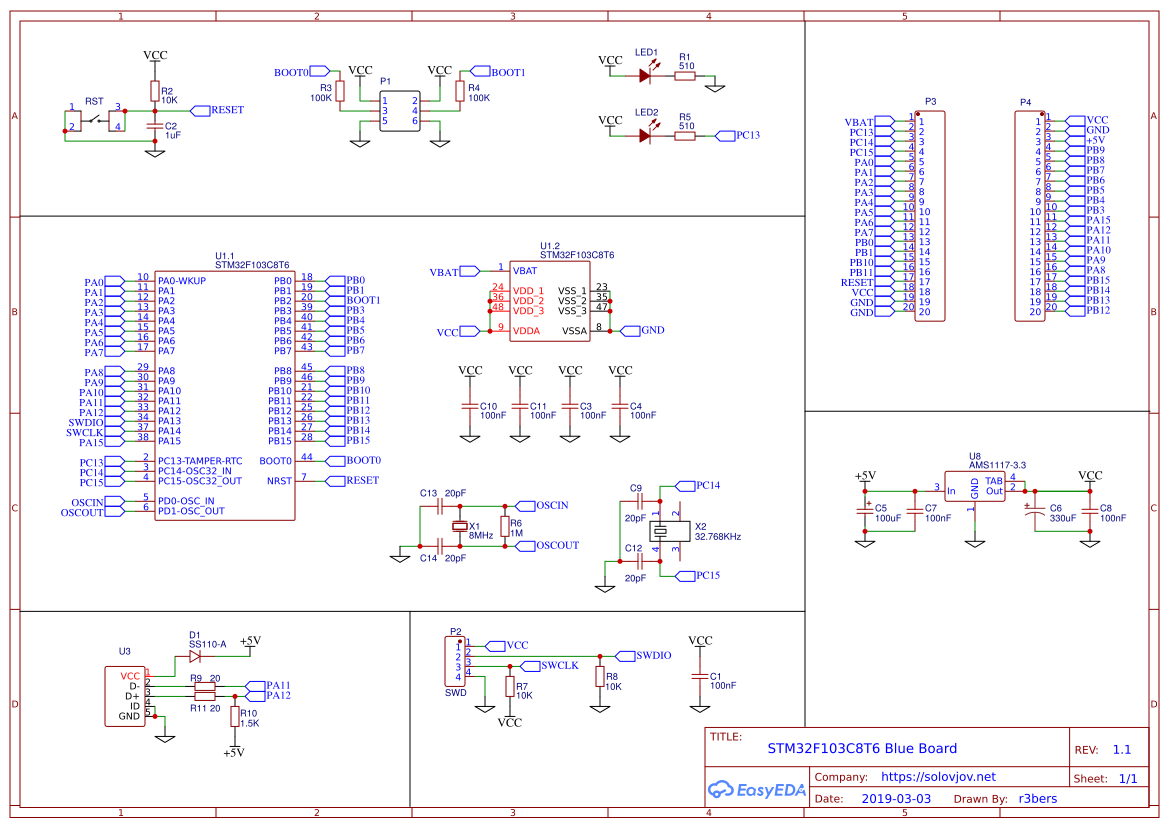
\includegraphics[scale=0.4]{images/esquematico_bluepill.png}
    \caption{Esquemático de Blue Pill}
	\label{fig:sch_bluepill}
\end{figure}
 % Seleccion de componentes 
\pagebreak

\chapter{Central de procesamiento}
\section{Descripción general}
\par El diseño general del sistema se pensó como tres nodos de escucha que son comandados y
procesados por medio de una central de procesamiento. Los requerimientos de la misma se
basan en las funcionalidades para establecer una comunicación estable y segura con cada uno
de los nodos, donde en caso de detectar una inhibición por parte de cualquier nodo requerir
el estado de los otros dos para así activar las alarmas correspondientes, comunicarse al
servidor web y volver a iniciar el sistema de cero una vez que se haya terminado el proceso
correctamente, dando también un reporte del estado de salud de cada nodo en particular.
\par En este capitulo se presentará la forma en que se llevo a cabo el desarrollo de la
misma, indicando su funcionamiento, primer prototipo, diseño final y la implementación de
un gabinete. 
\subsection{Funcionamiento}
\par El funcionamiento de la misma se podría dividir en tres partes interconectadas que se detallan 
a continuación.
\subsubsection{Comunicación con nodos}
\todo[inline]{poner referencias a sección de comunicación rs y con sim800}
\par Como ya se detallo en el apartado \ref{com_rs485}, la comunicación optada para la interconexión 
de los 4 dispositivos es RS485 por su forma de transmisión diferencial y largo alcance. 
\par Al inicio del sistema la central (funcionando como el maestro en la comunicación) requiere 
el estado de cada uno, del cual si detecta una inhibición alguno de ellos comenzaría el proceso 
para ver los demás nodos y comenzar a activar alarmas.

\subsubsection{Alarmas locales}
\par Una vez detectada la inhibición y procesado el estado del sistema en general, se dan las 
alarmas visuales y sonoras en la central misma para dar aviso al personal de seguridad que se 
encuentra en el lugar. 

\subsubsection{Comunicación remota al servidor web}
\par Como ya vimos en el apartado \ref{sim800}, la comunicación con el servidor web se hace de 
manera remota mediante GPRS una vez que se encuentra el sistema en un estado de alarma, cargando 
en el mismo la ubicación, ID de nodos, entre otros que se detallaran en las siguientes secciones. 

\section{Prototipo}
\subsection{Diseño}
\subsubsection{PCB}
\par En la figura \ref{im:pcb-prototipo} podemos ver una vista superior (izquierda) e inferior 
(derecha) de la placa prototipo para llevar a cabo la implementación de esta. 
\begin{figure}[h!]
\begin{center}
    \subfigure{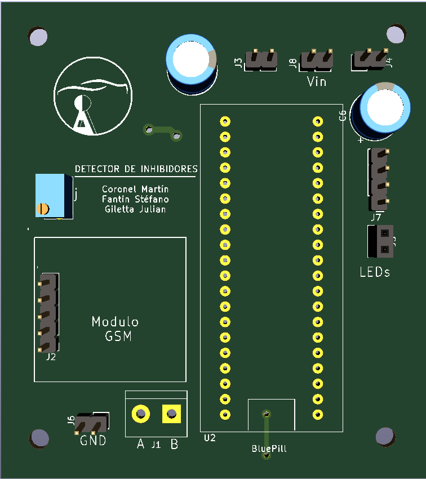
\includegraphics[width=60mm]{images/central/placa-prot-central-superior.png}}
    \subfigure{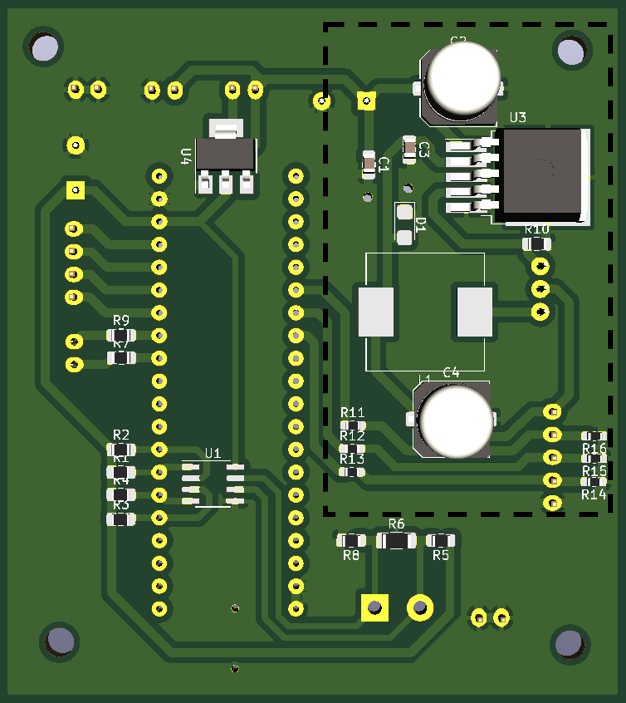
\includegraphics[width=60mm]{images/central/placa-prot-central-inferior.png}}
    \caption{Prototipo de placa de la central de procesamiento.}
	\label{im:pcb-prototipo}
\end{center}
\end{figure}

\subsection{Problemas surgidos}
\par Los principales problemas de esta primera aproximación al diseño final fueron en
base a la alimentación requeridas por el integrado de comunicación GPRS.
\par En primer lugar, era necesario un capacitor en la alimentación del SIM800 para
suavizar el arranque del mismo, ya que al conectarse a una red GSM/GPRS requiere un pico
de corriente de 2A.
\par Por otra parte, al tener que rediseñar la placa, notamos que la fuente conmutada implementada 
(encerrada en lineas cortadas en la figura \ref{im:pcb-prototipo}) requería gran cantidad de 
componentes, aumentando así el costo, principalmente con el integrado e inductor necesarios. 
Por ello, se opto como solución un regulador lineal con tan solo dos capacitores y dos resistencias 
se obtienen los requerimientos pedidos. 

\section{Diseño final}
\subsection{Software}
\par Para no volver redundante la explicación respecto del prototipo, se opto que el
funcionamiento del sistema embebido se detalle en esta sección ya que en cuanto a este no
fueron grandes los cambios realizados. 
\par En este apartado se nombraran como se llevaron a cabo los siguientes items:
\begin{itemize}
    \item Comunicación con nodos
    \item Salud de nodos
    \item Alarma sonora y visual
    \item Subida de datos al servidor web
\end{itemize}

\subsubsection{Comunicación con nodos}
\par Comenzamos nombrado esta etapa ya que es la tarea mas importante que ocurre en el dispositivo, 
un buen esquema de comunicación determina el buen funcionamiento del sistema en fin ya que, si bien 
los nodos son los encargados de detectar las inhibiciones, la central es el maestro que activa o no
 las alarmas y avisos. 
\par Para entender el funcionamiento podemos ver la imagen \ref{im:maq-est-central} en donde se 
observan 3 columnas correspondientes cada una a un estado de funcionamiento.
Como ya se nombro en la sección \ref{com_rs485}, la comunicación RS485 es half-duplex y debe existir
 un dispositivo maestro (en nuestro caso es el que se esta desarrollando), el cual es el encargado 
 de generar requerimientos a cada dispositivo de la red y si es necesario esperar una respuesta de 
 estos. 
En el estado 0, la comunicación es continua y rige un ciclo de un requerimiento de nodo por ves. 
La palabra es de 2 bytes, donde el primero corresponde al ID del nodo requerido y el segundo indica 
el estado que ocurre, esperando una respuesta por parte del nodo de una trama de 3 bytes designada 
de al forma que el primer byte corresponde nuevamente al ID del nodo, el segundo byte en este caso 
es 0 y el tercero el nodo reporta su estado de inhibición (0 para decir que no detecto inhibición, 
1 y 2 para alertar a la central que hay una inhibición ocurriendo). En caso de que el tercer byte 
de respuesta sea distinto de 0, pasaremos al estado siguiente.
\par En el estado 1, los requerimientos nuevamente es de un nodo a la vez y solo se volverá a 
ejecutar en el momento que un nodo no responda y deba chequear que solo fue una desincronización 
o que este se encuentre fallando. Aquí la palabra que envía la central es de 2 bytes indicando en 
el primero el ID del nodo y en el segundo un 1, correspondiente al estado que se encuentra, esperando
 recibir una respuesta de cada nodo con 3 bytes (ID de nodo, valor de RSSI medido y estado de 
 inhibición). Al tener la respuesta o no de cada nodo se actualizan las banderas de presencia de 
 inhibición, salud de los nodos, comienza la activación de alarmas y carga de datos al servidor web.

\par Posterior al comienzo de carga de datos al servidor, se pasa al estado 2 el cual envía repetidas
 veces en poco tiempo la palabra de 2 bytes "A2" correspondiente al reset del sistema para volver a 
 ponerse en modo de escucha y comenzar el ciclo nuevamente. 

\begin{figure}[h!]
	\centering
	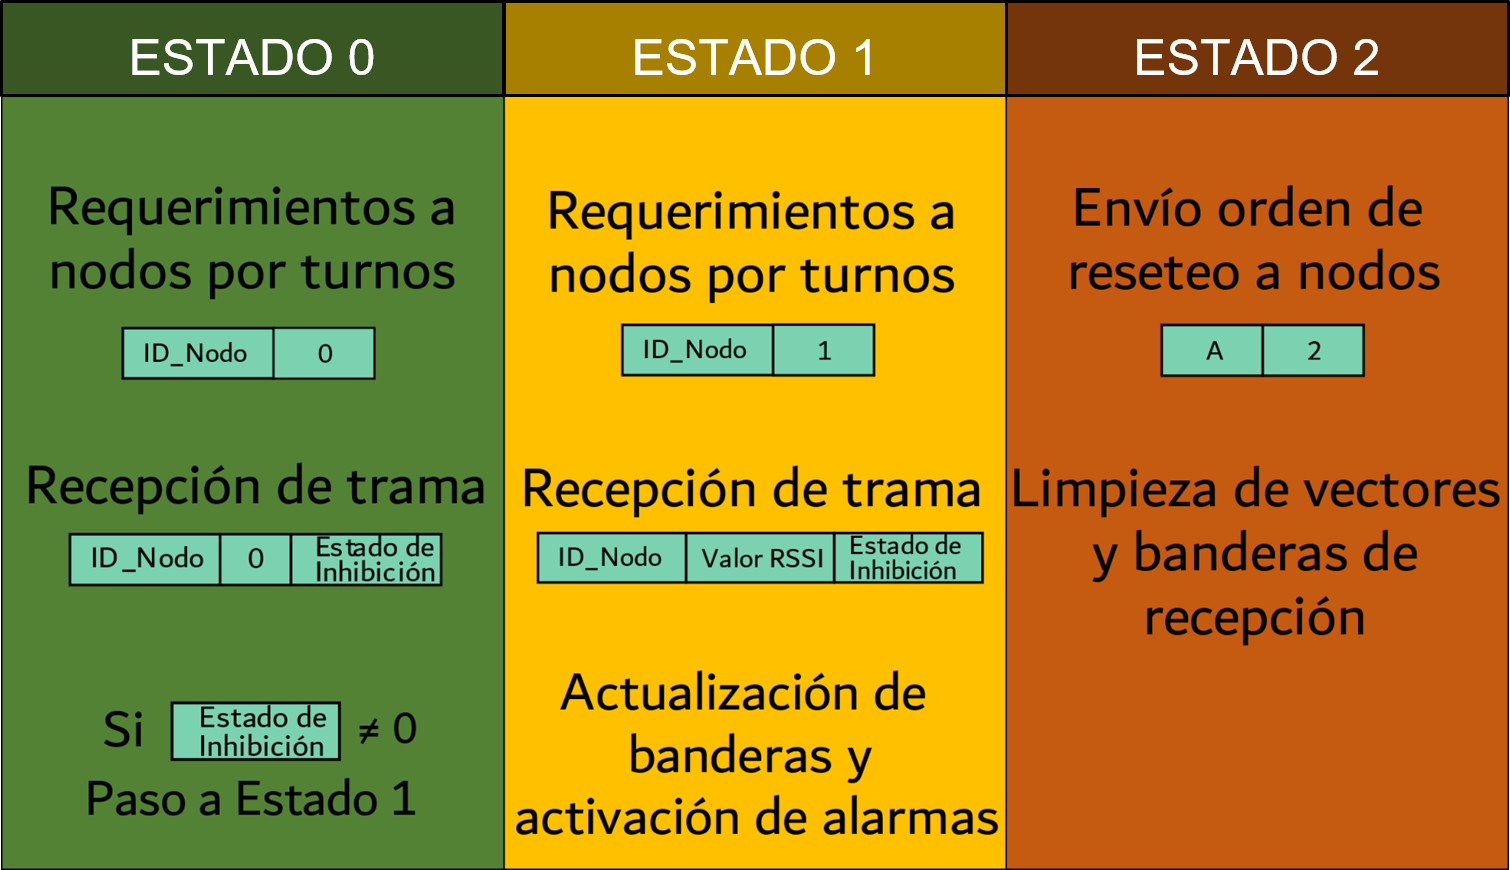
\includegraphics[scale=.53]{images/central/maquina-estado-central.png}
    \caption{Estados de la central en comunicación con nodos.}
	\label{im:maq-est-central}
\end{figure}


\subsubsection{Salud de nodos}
\par La salud de los nodos es un dato muy importante para saber que el sistema no falle, por ello 
la central tiene 3 leds en la parte frontal que indican si alguno no esta contestando los 
requerimientos pedidos, los cuales actualizan su estado en cada ciclo permitiendo así una 
visualización en tiempo real de la misma. 

\subsubsection{Alarma sonora y visual}
\par Localmente, al haberse activado las alertas de inhibición presente se activa un indicador 
lumínico en la central y además un pitido de 1 segundo para avisar al personal de seguridad o a 
la persona a cargo el hecho que ocurre. 

\subsubsection{Subida de datos al servidor web}
\par El enfoque que se le quiso dar a este sistema en general es la posibilidad de generar una base 
de datos de acceso remoto, no solo para poder triangular la posición en caso de ser posible, sino 
también pensando en que se pueda disponer este tipo de dispositivos en diferentes zonas y así generar 
estadísticas que tenga acceso cualquier persona y alertar sobre este tipo de episodios. 
\par El desenlace de cargar los datos remotamente via GPRS se da al fin del ciclo de detección.
 En este caso pasa algo particular, donde el integrado utilizado requiere que se le envien una serie
  de comandos para ser ejecutada cada acción y a su ves cada uno de ellos se puede enviar cada cierto
   tiempo. Por ello, para que el sistema no se congele cargando datos y dejando de escuchar los 
   canales de 433.92MH, esta carga se realiza en una interrupción del sistema, con los comandos a 
   enviar cargados por DMA (direct memory access) y los retardos necesarios son generados por la 
   cuenta de ticks (pulsos que se dan en el sistema cada 1ms) que no interrumpen la ejecución del 
   código, permitiendo que mientras se cargan los datos, también se reinicie el sistema y se siga 
   escuchando el canal por una nueva presencia de inhibición. 
\par La carga se realiza mediante un proceso de HTTP POST, la cual se realiza a traves de un 
formulario HTML, donde se le pasan los atributos necesarios para establecer el formato a cargar,
 en este caso se configura como "application/x-www-form-urlencoded", el cual indica que los datos 
 se pasan en forma de tuplas llave-valor separadas por '&' y un '=' entre la llave y el valor. Un 
 ejemplo de como se vería la carga es:
\begin{lstlisting}
    POST / HTTP/1.1 
    Host: www.jammer-detector.ml
    Content-Type: application/x-www-form-urlencoded 
    Content-Length: 19
    
    RSSI=45&mode_inhi=1 
\end{lstlisting}
\subsection{Hardware}
\par En este apartado se mostrara una descripción de la placa que contiene el MCU, los esquemáticos 
finales, el pcb obtenido y su modelo en 3D. 


\subsubsection{Esquemático}
\par Como en el apartado de selección de componentes se ha explayado, como microcontrolador se hace 
uso del STM32F106C8T6. Este 
cuenta con un cristal de 8 MHz, el cual mediante un PLL interno es llevado a la frecuencia de 
operación de 72 MHz. En la
figura \ref{cristal_bluepill} se puede observar lo antes mencionado.

\begin{figure}[!h]
	\centering
	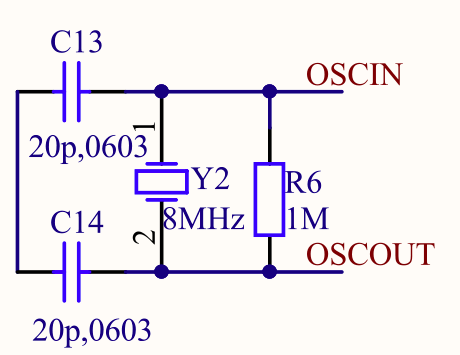
\includegraphics[scale=0.35]{images/central/bluepill-osc.png}
    \caption{Cristal para el MCU}
	\label{cristal_bluepill}
\end{figure}

\par También cuenta con un regulador de 5V a 3.3V (figura \ref{im:reg-bluepill}) para la alimentación
 a los pines que manejan estos niveles de lógica y es utilizado también para el debugger. Por ultimo
  como se observa en la figura \ref{im:reset-bluepill}, la placa tiene un botón de reset el cual es 
  activo por bajo. 

\begin{figure}[!h]
	\centering
	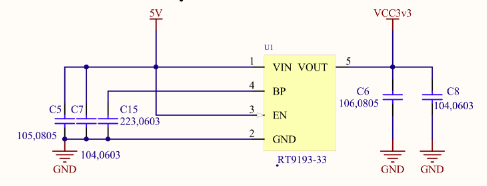
\includegraphics[scale=0.6]{images/central/bluepill-reg.png}
    \caption{Regulador de 5V a 3.3V para MCU.}
	\label{im:reg-bluepill}
\end{figure}

\begin{figure}[!h]
	\centering
	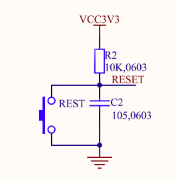
\includegraphics[scale=0.6]{images/central/bluepill-reset.png}
    \caption{Reset de microcontrolador.}
	\label{im:reset-bluepill}
\end{figure}

\par El esquemático en general se separo en varias partes para que se puedan observar de una manera 
mas ordenada en el presente informe. Estas 3 partes nombradas se pueden ver en las figuras 
\ref{im:esq-central-1}, \ref{im:esq-central-2} y \ref{im:esq-central-3} con su descripción de la 
correspondencia de cada una de ellas. 

\begin{figure}[!h]
	\centering
	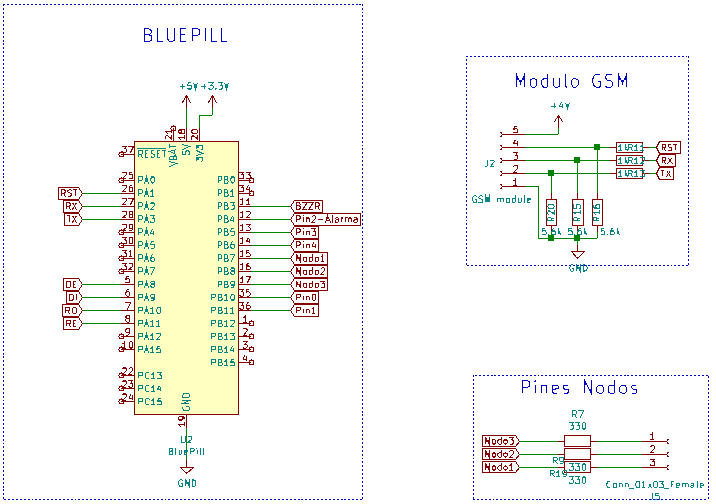
\includegraphics[scale=.50]{images/central/central-esq-1.png}
    \caption{MCU, modulo GSM/GPRS y leds indicadores de nodos.}
	\label{im:esq-central-1}
\end{figure}

\begin{figure}[!h]
	\centering
	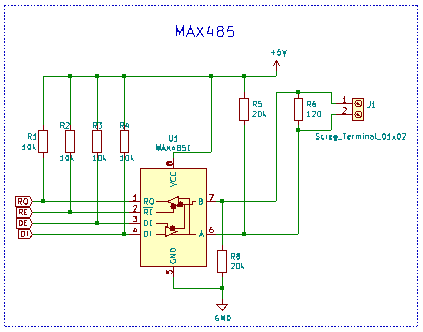
\includegraphics[scale=.59]{images/central/central-esq-2.png}
    \caption{Sección de comunicación RS485.}
	\label{im:esq-central-2}
\end{figure}

\begin{figure}[!h]
	\centering
	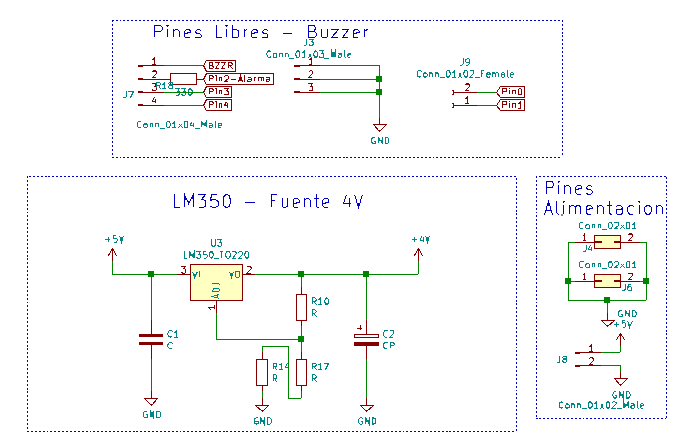
\includegraphics[scale=.55]{images/central/central-esq-3.png}
    \caption{Pines de alimentación, regulación para SIM800 y pines libres para conexiones adicionales.}
	\label{im:esq-central-3}
\end{figure}

\subsubsection{PCB}
En la figura \ref{im:pcb-final} vemos el diseño final de la placa de la central, el cual se diferencia 
al prototipo (figura \ref{im:pcb-prototipo}) en la fuente conmutada, que fue reemplazada por una 
lineal y en la adición de los leds indicadores de estado de cada nodo. 

\begin{figure}[!h]
\begin{center}
    \subfigure{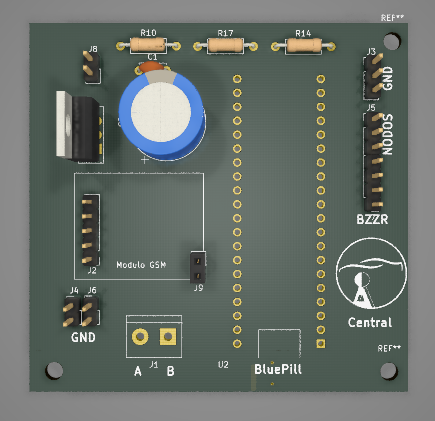
\includegraphics[width=60mm]{images/central/Central top.png}}
    \subfigure{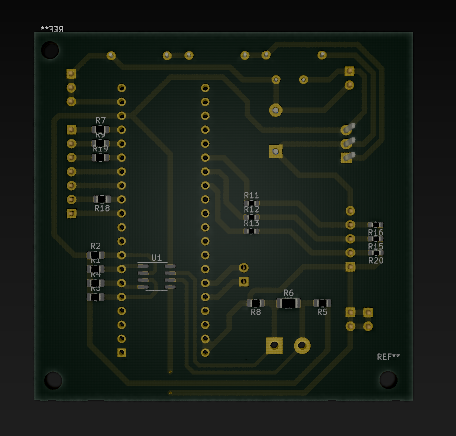
\includegraphics[width=60mm]{images/central/central-botton.png}}
    \caption{Diseño final de placa de la central de procesamiento.}
	\label{im:pcb-final}
\end{center}
\end{figure}

\subsubsection{Modelo 3D}
El modelo 3D de la placa la podemos observar en la figura \ref{im:mod-3d-central}.

\begin{figure}[!h]
	\centering
	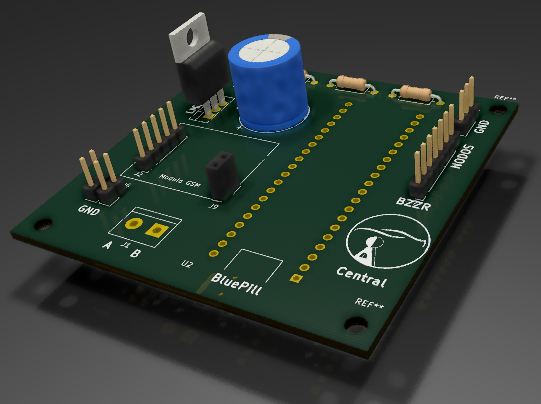
\includegraphics[scale=.55]{images/central/Central-perspectiva.png}
    \caption{Vista en 3D de la placa final de la central de procesamiento.}
	\label{im:mod-3d-central}
\end{figure}

\section{Gabinete}
\par El diseño del gabinete (figura \ref{im:gabinete-central}) de la central se busco que fuera de 
una forma vertical, en donde por delante se observen cinco indicadores lumínicos que informar sobre
 el estado de inhibición del sistema (agregado de un buzzer también), el estado de salud de cada nodo
  y si esta en funcionamiento o no.
\par Por la parte trasera encontramos un interruptor para alimentar a todos los nodos, conector para
 12V y un conector GXS para la comunicación RS485 y llevar la alimentación a cada nodo bajo el 
 concepto de power over ethernet. 
\begin{figure}[!h]
\begin{center}
    \subfigure{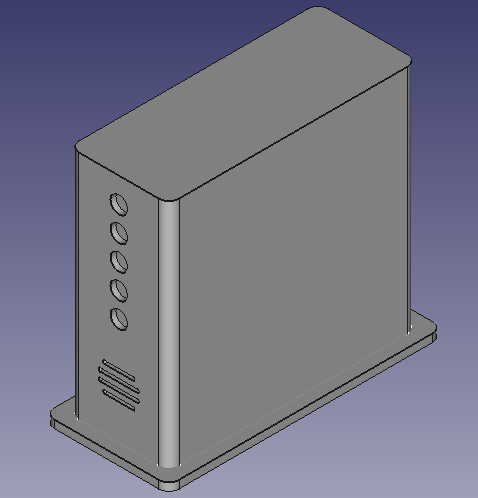
\includegraphics[width=55mm]{images/central/modelo-3d-central-frente.png}}
    \subfigure{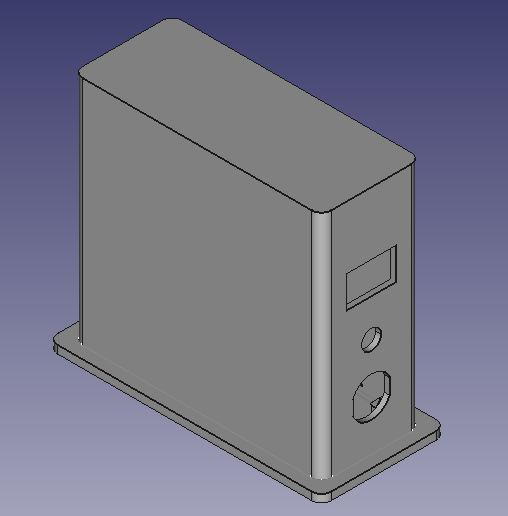
\includegraphics[width=56mm]{images/central/modelo-3d-central-atras.png}}
    \caption{Gabinete de central armado.}
	\label{im:gabinete-central}
\end{center}
\end{figure}

\par El mismo se llevo a la realidad por medio de impresión 3D en plástico PLA negro. Para comodidad
 en el armado e impresión, vemos en la figura \ref{im:impresion-central} que el modelo se dividió 
 en 2 partes, donde una llamada "base" es la encargada de soportar la placa principal de la central 
 y en la parte de la derecha, que denominamos "tapa", encontramos los indicadores y demás conectores.
 

\begin{figure}[!h]
	\centering
	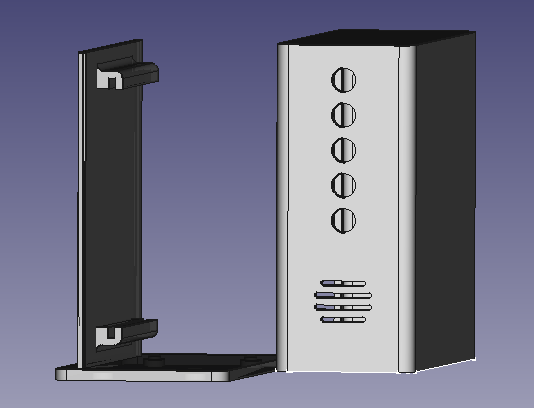
\includegraphics[scale=.53]{images/central/modelo-3d-central-separado.png}
    \caption{Partes para el armado del gabinete de central.}
	\label{im:impresion-central}
\end{figure}
 % Central
\pagebreak

\chapter{Nodos de recepción} \par 

\section{Descripción general}

En este capítulo haremos un análisis profundo sobre el funcionamiento de los nodos en el sistema de detección de inhibidores
de alarma de autos. Para comenzar con el mismo es importante preguntarse: ¿qué funciones debe cumplir un nodo en el sistema?
La respuesta a esto es evidente, en el nodo se producirá la recepción de la señal de RF mediante el módulo CC1101 de Texas 
Instruments, luego de esto la demodulación ASK efectuada por el receptor será procesada en el microcontrolador seleccionado
para determinar si hay o no inhibición según estrategias más adelante detalladas y este se encargará de realizar la 
comunicación mediante el protocolo RS485 con la central de procesamientos. Integrado en el nodo se utilizan tres protocolos 
de comunicación: en primer lugar tenemos la comunicación SPI que se encarga de la interacción entre el microcontrolador y 
el receptor seleccionado; esta comunicación se utiliza para configurar los registros del CC1101 para establecer el modo de
trabajo deseado. En segunda instancia tenemos comunicación serial asíncrona entre un pin de salida del receptor por el cual 
se mandan los datos RAW de demodulación en el canal seleccionado y en último lugar tenemos el protocolo RS485 para la comunicación
de la red armada. 

\section{Prototipo}

El proceso de obtener un sistema sólido y que responda a las necesidades planteadas llevó consigo la necesidad de elaborar
dos modelos distintos de nodo. En un comienzo se buscó que el mismo tenga una realimentación visual de las mediciones tomadas,
por lo que, además de procesar las señales mediante las estrategias de detección establecidas, se asignaron salidas en seis leds
que se encargaban de indicar la potencia de RF medida con el RSSI como se puede observar en la figura \ref{prototipo_nodo}. \par 

\begin{figure}
	\centering
	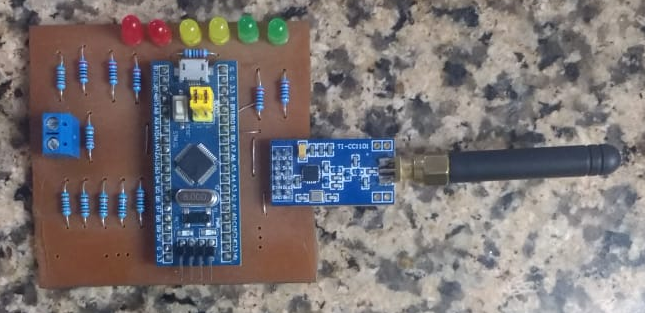
\includegraphics[scale=0.53]{images/nodos/prototipo_nodo.png}
    \caption{Primer placa del nodo armada}
	\label{prototipo_nodo}
\end{figure}

Visualmente el prototipo es bastante rudimentario, las placas fueron fabricadas de manera casera y sin tener grandes
cuidados en los detalles. De igual modo este diseño bastó para pulir las imperfecciones que poseía en camino al desarrollo final.\par 
Para el diseño del esquemático nos hemos basado en las prestaciones que nos brinda el microcontrolador STM32F106C8T6. El mismo
cuenta con comunicación SPI y serial integradas, por lo que haciendo uso del entorno de programación propio del fabricante 
(STM32 Cube IDE) hemos asignado los pines respectivos a cada comunicación, como muestra la figura \ref{asignacion_pines}. \par

\begin{figure}
	\centering
	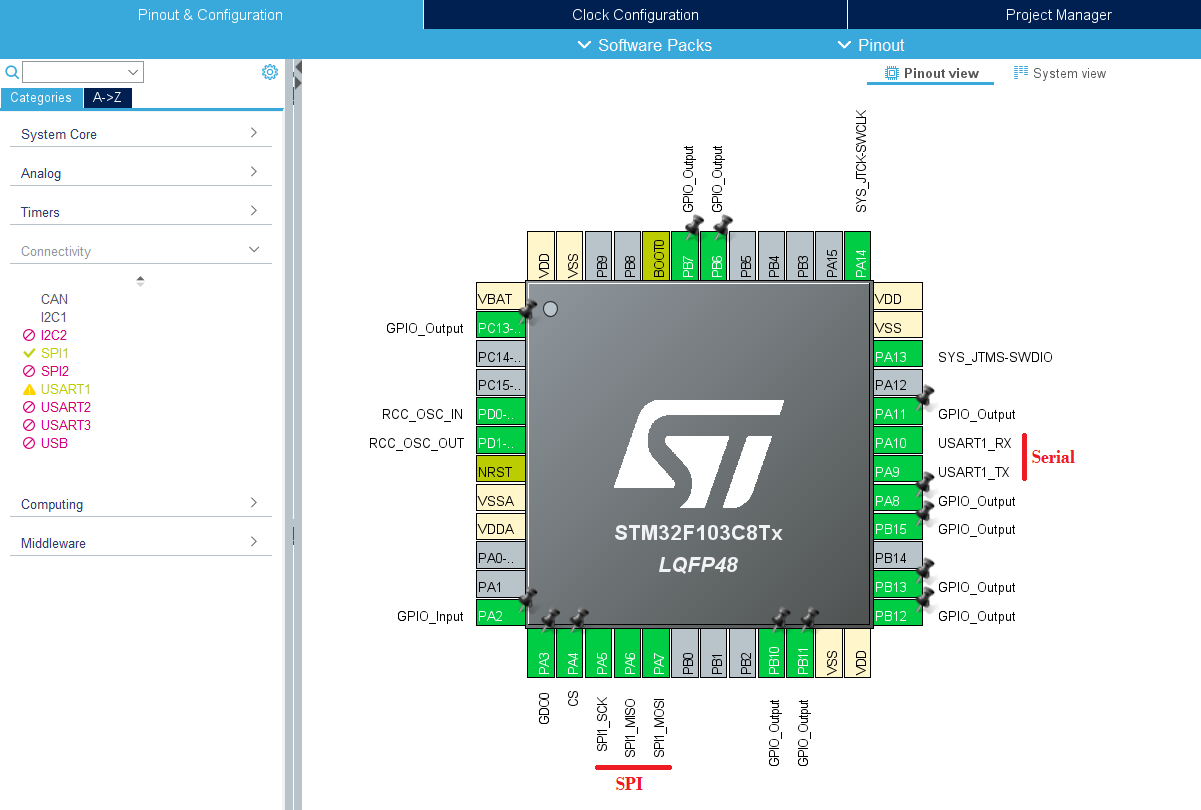
\includegraphics[scale=0.43]{images/nodos/asignacion_pines.png}
    \caption{Asignación de pines para comunicación}
	\label{asignacion_pines}
\end{figure}

Trabajar con este entorno es muy beneficioso ya que facilita en algunos aspectos la configuración del microcontrolador 
seleccionado, teniendo la capacidad de, mediante una interfaz gráfica, activar comunicaciones, configurar los relojes,
activar o desactivar interrupciones de timers y comunicaciones, entre otras. \par 
Las interrupciones en nuestro diseño juegan un papel clave debido a que en la comunicación se ha optado en algunos casos
particulares realizar el envío de los datos mediante interrupciones para que el procesador pueda continuar operando y no aboque 
todos sus recursos y tiempo de ejecución en enviar una palabra. De modo similar las interrupciones de timers nos han servido
para realizar acciones con alta prioridad y que deben ejecutarse en un tiempo específico, como por ejemplo la lectura asíncrona
de datos RAW enviados por un pin del CC1101. La configuración para las mismas se realiza de manera muy sencilla teniendo en 
cuenta el contador de ticks del sistema, la frecuencia del clock utilizada y un preescaler a determinar para lograr el tiempo
deseado. \par 

\section{Diseño final}

El diseño el nodo ha surgido ciertas variaciones en el transcurso de la búsqueda del producto final. Entre estas se encuentra
la optimización del PCB reduciendo el tamaño del mismo, retirar los indicaores led y dotar la placa con el integrado destinado 
a la comunicación (SN75176). Para hacer un anális particular del funcionamiento del nodo hemos decidido analizar independientemente
el software del hardware.

\subsection{Software}

El nodo al ser el encargado de recibir la señal de RF, demodularla y determinar si hay o no inhibición posee una alta carga 
de software desarrollado sobre él. De este modo señalaremos particularmente el desarrollo en cada uno de los siguientes 
aspectos.

\begin{itemize}
	\item Recepción de RF.
	\item Estrategia de detección de inhibiciones.
	\item Comunicación con la central.
\end{itemize}

\subsubsection{Recepción RF}

El desarrollo de software en este aspecto cumple la necesidad que presenta el integrado receptor que utilizamos de ser 
configurado cada vez que este comienza a operar. Como previamente es analizado debemos establecer al dispositivo, que por
características es un transceptor, en modo de recepción. Además se debe configurar la frecuencia de operación, el modo de 
demodulación, el tipo de salida de datos, entre otras muchas cosas que son cargadas en un total de 46 registros. \par 
La carga de registros y los requerimientos de valor de RSSI que se le producen al CC1101 para tener noción de la potencia 
de RF en dBm que está llegando al receptor se realizan mediante comunicación SPI. Estos requerimientos son periódicos y 
han sido establecidos con un tiempo prudencial para que la comunicación resulte efectiva y los datos permanezcan actualizados.

\subsubsection{Estrategia de detección de inhibiciones}

La estrategia de detección de inhibiciones ha sido uno de los mayores desafíos a la hora de encarar el proyecto a causa de que
el sistema debe ser confiable y robusto para poder instalarlo en una zona de operación y que no tenga fallos. Principalmente
los errores de funcionamiento que son inadmisibles son: 
\begin{itemize}
	\item Falsas detecciones: que el sistema desate las alarmas cuando no hay presente un inhibidor o cuando en el canal se está
	comunicando un dispositivo que sí es apto para hacerlo, como por ejemplo una llave de auto.
	\item Falsos negativos: que el sistema sea incapaz de reconocer una señal que sea perjudicial para el sistema de seguridad
	de un automóvil.
\end{itemize} 

Antes se ha profundizado en las estrategias de inhibición y se ha llegado a la conclusión de que existen dos métodos posibles
para inhibir una comunicación, un método es saturación de la etapa receptora y el otro es por corrupción de la trama de datos.
Para ambos métodos se ha debido realizar una estrategia de detección diferente, las cuales funcionan en simultáneo en el nodo
para desatar las alertas correspondientes si detectaran positivo. A continuación en las figuras \ref{estrategia_rssi} 
y \ref{estrategia_datos} se demuestra en bloques el funcionamiento de la estrategia de detección.

\begin{figure}
	\centering
	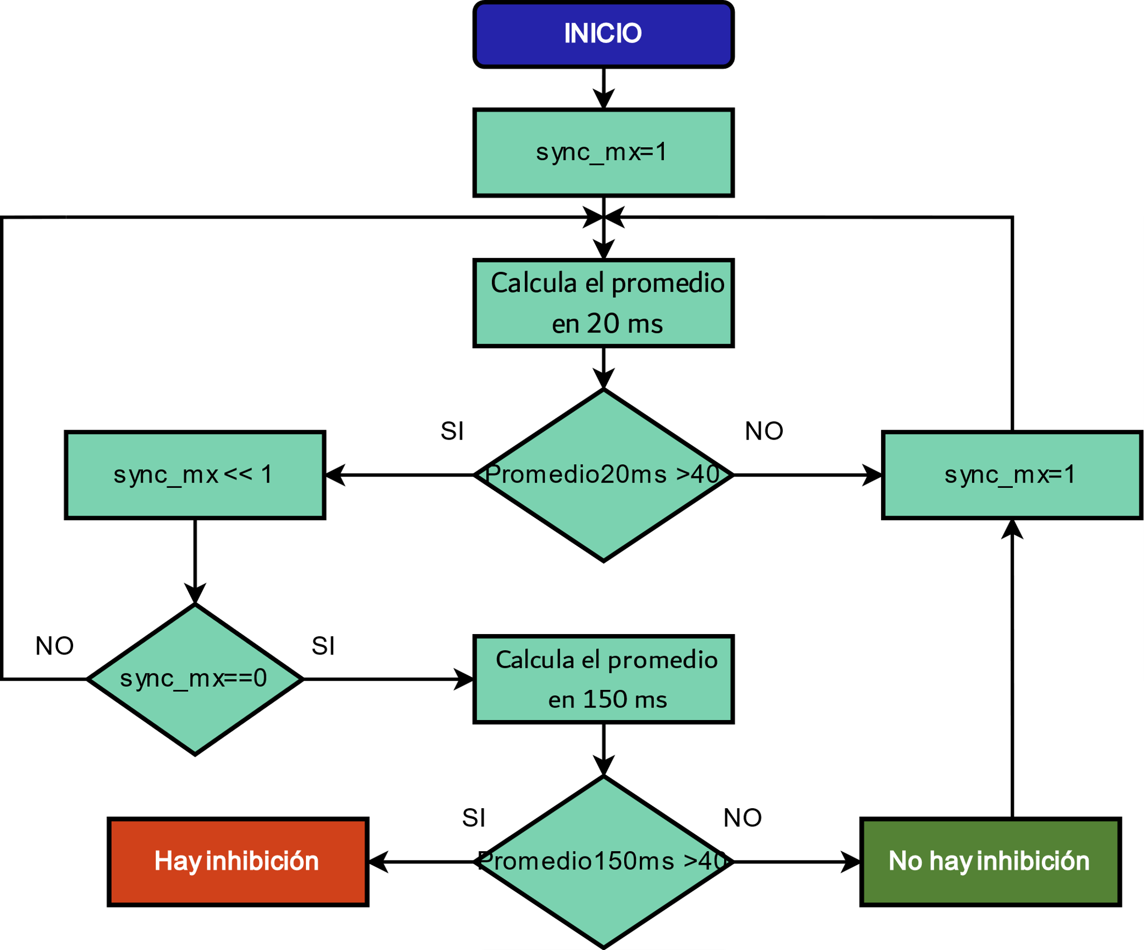
\includegraphics[scale=0.43]{images/nodos/estrategia_datos.png}
    \caption{Estrategia de detección por corrupción de datos}
	\label{estrategia_datos}
\end{figure}

\begin{figure}
	\centering
	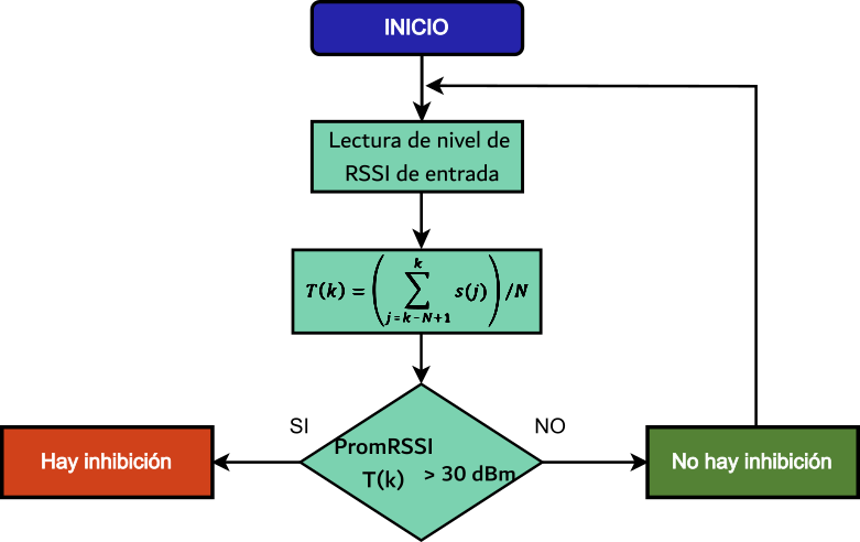
\includegraphics[scale=0.43]{images/nodos/estrategia_rssi.png}
    \caption{Estrategia de detección por saturación de etapa receptora}
	\label{estrategia_rssi}
\end{figure}

\subsubsection{Comunicación con la central}

Para el corriente funcionamiento del sistema se precisa que los nodos se mantengan comunicados a la central, dando información  
de lo que cada uno están recibiendo y esta encargándose de manejar las alertas y los requerimientos a cada uno de los 
receptores. \par 
Para que la comunicación sea lo más efectiva posible se decidió que respete siempre una estructura de comunicación constante
en la que únicamente se cambirán los parámetros a enviar. La comunicación es del tipo master -la central- esclavos -los nodos-
y cada uno de los esclavos responderán por turno con peticiones independientes. \par
Como antes se mencionó la trama de comunicación es única y puede observarses en la figura \ref{comunicacion_nodo}, donde 
ID Nodo hace referencia al identificador propio del nodo en la red, Valor RSSI al valor de intensidad de señal recibido por cada
nodo y Estado hace referencia al estado de inhibición detectado, siendo 0 para no inhibición, 1 para inhibicion por corrupción
de datos y 2 para inhibición por saturación.

\begin{figure}
	\centering
	
\includegraphics[scale=0.43]{images/nodos/comunicacion_nodo.png}
    \caption{Estados de comunicación en nodo}
	\label{comunicacion_nodo}
\end{figure}


\subsection{Hardware}

En el nodo de recepción se hace uso del mismo MCU que en la central, de modo que las características de hardware antes mencionadas
tienen completa validez aquí también. Comunicado por SPI y comunicación serial se encuentra el módulo CC1101, luego mediante
comunicación serial asíncrona tenemos el SN75176. En la figura \ref{schema_nodo} podemos observar los tres bloques principales
que lo componen. \par 


\begin{figure}
	\centering
	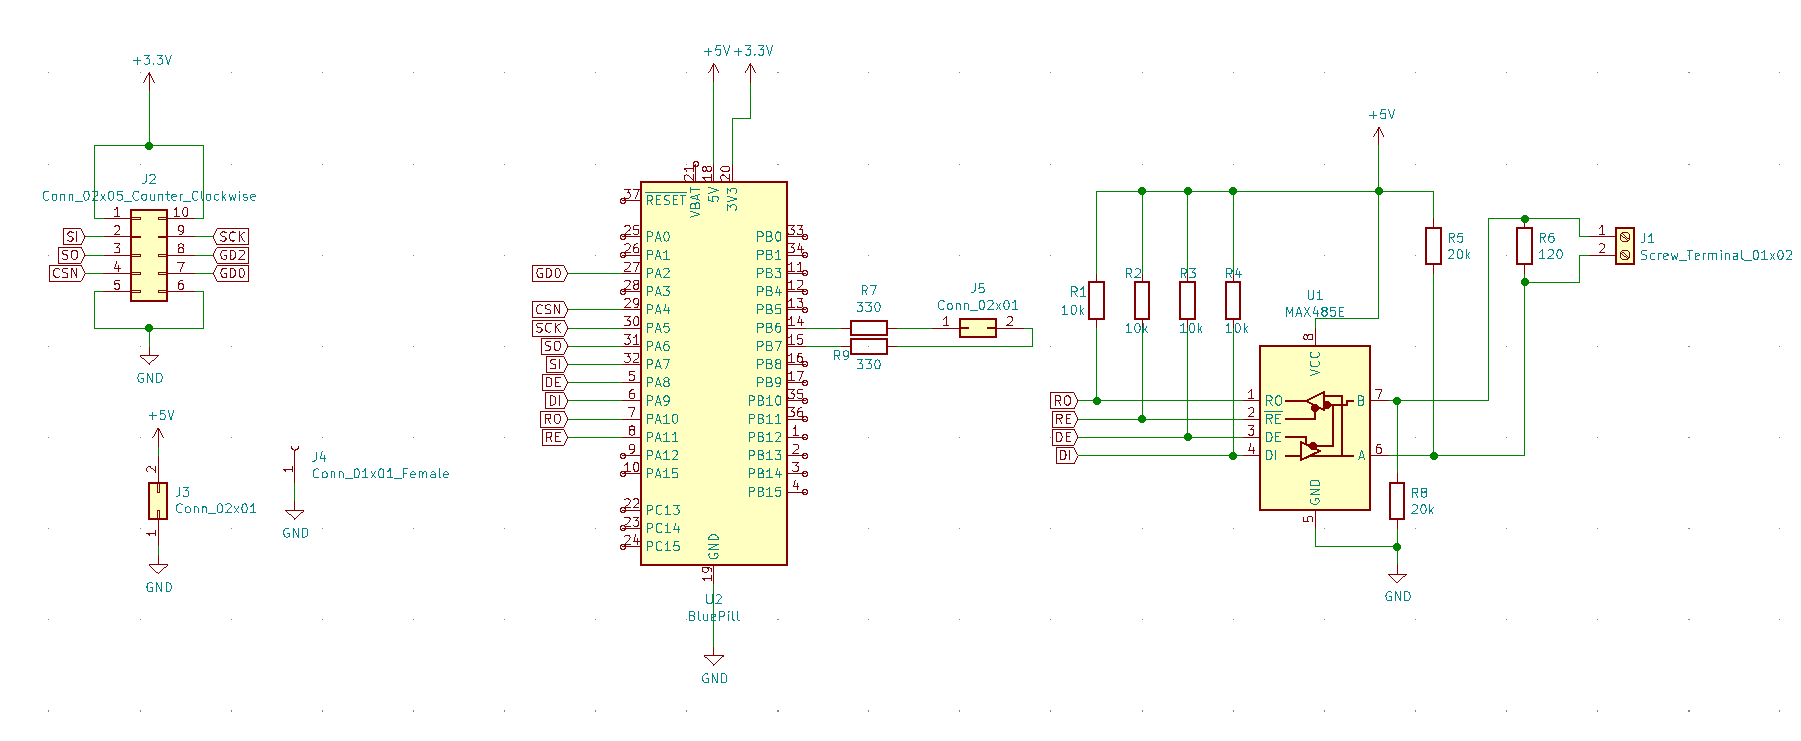
\includegraphics[scale=0.3]{images/nodos/schema_nodo.png}
    \caption{Esquemático del nodo receptor}
	\label{schema_nodo}
\end{figure}

Tenemos de derecha a izquierda en el esquemático los pines de conección del CC1101, el cual está unido al MCU por seis pines, los 
cuales pueden ser seguidos por las etiquetas que este y el microcontrolador poseen y por último tenemos el esquemático para 
la comunicación RS485. \par 

El diseño 3D de la placa terminada se puede ver en la figura \ref{3d_nodo}. En las perforaciones que se observan van 
instalados los módulos utilizados que en el apartado de selección de componentes se mencionan.


\begin{figure}[!h]
	\begin{center}
		\subfigure{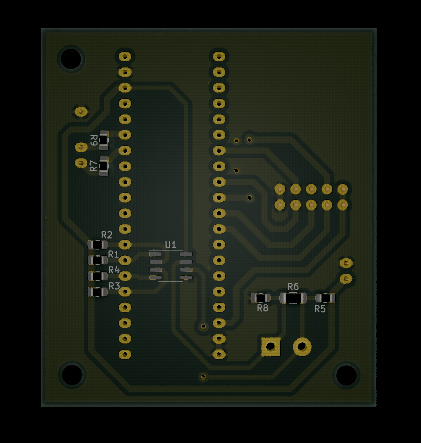
\includegraphics[width=60mm]{images/nodos/nodo-botton.png}}
		\subfigure{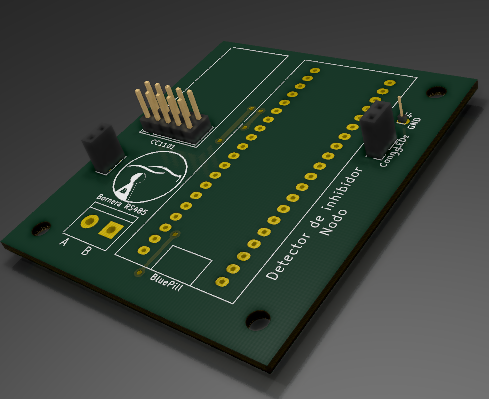
\includegraphics[width=60mm]{images/nodos/nodo-perspectiva.png}}
		\caption{Diseño 3D del nodo receptor.}
		\label{3d_nodo}
	\end{center}
\end{figure}


\subsection{Gabinete}

El diseño del gabinete del nodo fue realizado con un diseño minimalista y con características cúbicas, separado en tres secciones que facilitan
la impersión y el armado. El diseño terminado se muestra en la imagen \ref{gabinete_nodo}. \par 
EL gabinete no posee realimentación visual del estado 
de funcionamiento, a simple vista es un cubo flotante con la antena de 433,92MHz asomando por uno de sus lados al que se ha buscado que no 
sea visible de qué manera ingresan los cables y la ficha GXS al sistema, para mayor estética. Está impreso en PLA negro, al igual que la central de 
procesamientos y tiene orificios para cuatro tornillos de modo que pueda ser instalado en una superficie plana.  \par 

\begin{figure}[!h]
	\begin{center}
		\subfigure{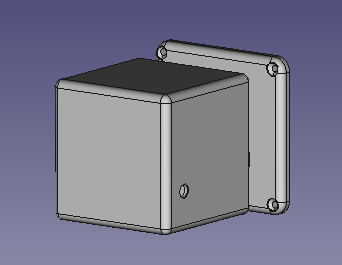
\includegraphics[width=60mm]{images/nodos/modelo-3d-nodo.png}}
		\subfigure{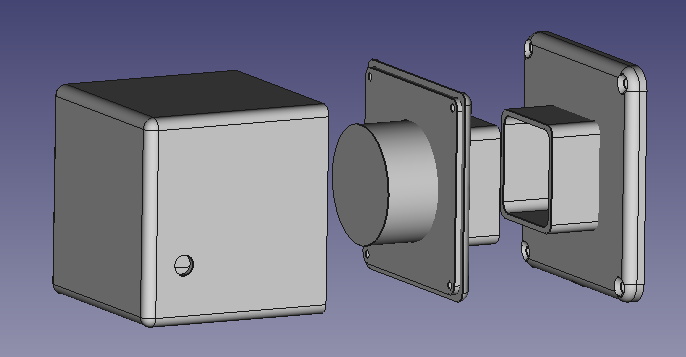
\includegraphics[width=60mm]{images/nodos/modelo-3d-nodo-3partes.png}}
		\caption{Gabinete del nodo receptor terminado.}
		\label{gabinete_nodo}
	\end{center}
\end{figure}

 % Nodos
\pagebreak

\chapter{Ensayos}

En este capítulo hablaremos sobre los ensayos que se han realizado a lo largo del desarrollo del proyecto. Se llevaron a cabo diversas pruebas
sobre las diferentes partes que componen el sistema, en cada sección de este capítulo se exponen los ensayos realizados a cada una de esas partes
o subsistemas.

\section {Análisis de llaves e inhibidores} 

El primer conjunto de ensayos que realizamos fueron enfocados a conocer la naturaleza de las comunicaciones de los sistemas de seguridad vehicular
y de los inhibidores. En esta instancia fue muy importante el uso de un SDR (Radio definida por software) para analizar el espectro de las señales y
llevar a cabo la demodulación, como ya explicamos en la sección 1.1.2. \par 
Las primeras mediciones las realizamos a distintas llaves, como podemos observar en la figura \ref{llaves}. Los datos obtenidos mediante el SDR
fueron de gran importancia para conocer en profundiad la estructura de la comunicación de las llaves, información indispensable para establecer 
métodos de inhibición adecuados.
Como ya lo mencionamos en 1.1.3, hay dos tipos de inhibiciones, por lo cual fue necesario obtener al menos dos inhibidores que ataquen al sistema 
de seguridad de esas maneras. \par
El primer inhibidor que usamos consiste sencillamente en un handie (o transceptor de radio portátil) que es capaz
de emitir en la misma frecuencia que las llaves de los autos y debido a la potencia que posee logra saturar la etapa receptora de los automóviles.
Por otro lado, para lograr inhibir por corrupción de datos fabricamos nuestro propio inhibidor, el cual emite un tono de baja potencia dentro del ancho de banda
del receptor, logrando corromper la trama de comunicación.\par 

Los ensayos realizados con los inhibidores consistieron en conocer la vulnerabilidad de los sistemas de seguridad de los vehículos así como las
distancias y potencias que se requerían para inhibir. En el caso del handie, es capaz de lograr interferir en la comunicación de la llave y el auto a
distancias grandes debido a su alta potencia, mientras que en el caso del inhibidor por corrupción de datos necesita situarce a distancias
cortas del vehículo. Esta información es muy importante para plantear un sistema realista y desarrollar una adecuada estrategia de detección.

\section {Pruebas y configuración del CC1101}

Una vez analizadas las características de las señales de interés con ayuda de un SDR estábamos listos para probar el integrado elegido para la
recepción. En este ensayo utilizamos la Blue Pill para configurar los registros del CC1101 mediante comunicación SPI.
La primer prueba consistió simplemente en constatar que la comunicación SPI funcionaba, esto se hizo configurando los registros con valores predeterminados 
y posteriormente requiriendo el valor de alguno de ellos desde la Blue Pill.\par 
Con la comunicación funcionando procedimos a encontrar los valores adecuados para los registros de configuración del CC1101.
Lo que se buscaba en este punto era configurar el integrado para que nos entregue la demodulación y el valor de RSSI de la señal que recibía, 
así como también dar con los valores adecuados de sensibilidad y ancho de banda. Para calcular los valores de los registros nos ayudamos del datasheet del CC1101
y del software SmartRF Studio, que recomienda el fabricante.

\section{Ensayos de las estrategias de detección}

En esta instancia ya éramos capaces de extraer los datos relevantes de la señal recibida y acceder a ellos mediante la Blue Pill, por lo que se procedió a
desarrollar un algoritmo que, mediante estos datos, pueda decidir si la señal recibida se trata de una interferencia emitida por un inhibidor.\par
En primer lugar se creó un mecanismo simple y, gracias a ensayos utilizando llaves y nuestros propios inhibidores, fuimos mejorando nuestras estrategias
de detección hasta volver al sistema confiable. La lógica de funcionamiento la podemos ver en las figuras \ref{estrategia_datos} y \ref{estrategia_rssi}\par 
Hasta ahora, la Blue Pll la utilizamos conectada a una computadora para poder debuggear los programas que ensayábamos y así encontrar fallos de forma
rápida. Sin embargo, en un producto final, debía ser capaz de actuar independiente, es por esto que en este punto desarrollamos el primer
prototipo de nodo, que ya mostramos en la figura \ref{prototipo_nodo}). Sobre este primer prototipo se realizaron diversos ensayos para terminar
de afinar la detección. \par

\section{Servidor Web y conexión a internet}

Paralelo al desarrollo del nodo trabajamos en contruir un sitio web propio capaz de recibir información y plasmarla en tablas y gráficos.
En una primera instancia se ensayó el servidor web subiendo datos de forma manual, lo que nos permtía ver como oganizaba y mostraba los datos. \par
Una vez funcionando bien el sitio web procedimos a realizar pruebas sobre el SIM800L. Recordemos que este módulo es el responsable de dar a la central conexión
a internet mediante 2G.
El SIM800L se comunica mediante comandos AT, por lo que lo usamos en conjunto con la Blue Pill para relizar los ensayos. En primer lugar solamente
buscábamos que el SIM800L logre conectarse a la red gracias a una SIM que le insertamos. Puede parece un paso simple, pero debido a que este módulo
posee requerimientos particulares en cuanto a la alimentación fue importante realizar pruebas para desarrollar una fuente adecuada para el mismo.
Cuando logramos que el SIM800L se conecte con la red ensayamos la capacidad que tenía de subir datos al servior mediante las órdenes recibidas desde 
la Blue Pill a través de los comandos AT.\par 

\section{Desarrollo de la comunicación serial del sistema}

En este punto ya logramos tener un nodo capaz de recibir señales y de detectar inhibiciones y un servidor web funcional al cual podemos subir datos
mediante el SIM800L y una Blue Pill. El siguiente paso, era desarrollar una comunicación robusta entre nodos y la central. Fue en este momento que decidimos
usar el MAX485 para comunicar el sistema mediante RS485.\par
Al añadir el MAX485 al conjunto de SIM800L y Blue Pill, queda conformado el primer prototipo en protoboard de nuestra central.\par
Los primeros ensayos consistieron simplemente en comunicar dos Blue Pill aisladas, esto era necesario para conocer el estandar de comunicación en cuestión
y familiarizarnos con el manejo de la UART del nuestro microcontrolador. El siguiente paso fue añadir el prototipo del nodo con el agregado de un max485
y nuestro prototipo de central. En este punto todavía no estábamos enviando datos de recepción a través de la comunicación, solamente envíabamos datos
sin importancia para entender como conformar un red de rs485. Estos ensayos nos permitieron desarrollar una estrategia de comunicación confiable.\par
Fue en este momento cuando desarrollamos nuestra trama de comunicación y, luego de varios ensayos, definimos por completo como se iban a comunicar los nodos
y la central. En este punto se realizaron numerosos ensayos del sistema funcionando en conjunto, desde la detección de la inhibición y la comunicación de los nodos
a la central, hasta encender alarmas y subir los datos a la web.
Cabe aclarar que todas las pruebas de comunicación realizadas hasta el momento se hicierona a cortas distancias con un par trensado telefónico.

\section{Ensayos Finales}

Al quedar ya conformado el formato de nuestro sistema, diseñamos nuestras placas definitivas y las mandamos a fabricar. Con nuestros nodos y la central
llevamos a cabo los últimos ensayos, esta vez utilizando un cable de mayor longitud y situándonos en un espacio de gran tamaño.
Gracias a estas pruebas realizamos los últimos ajustes para lograr un sistema robusto y funcional. \par
Por último se puso a pruebas el sistema en un estacionamiento real, obteniendo excelentes resultados.


 % Ensayos
\pagebreak

\chapter{Desarrollo de servidor web}
\section{Objetivos}
\section{Pagina web}
\subsection{Pestañas}
\subsubsection{Inicio}
\subsubsection{Nosotros}
\subsubsection{Estadísticas}
\subsubsection{Triangulación}
\subsubsection{Contacto}
\section{Base de datos}
\subsection{Contenido}
\subsection{Carga de datos} % Servidor web - Corregido
\pagebreak

\chapter{Conclusiones y trabajo futuro} \par

De acuerdo al trabajo previamente expuesto en este capítulo haremos mención de las conclusiones que pudimos extraer al 
finalizarlo y se evaluarán posibilidades de desarrollos futuros. \par

\section{Conlcusiones} \par 

En primera instancia nos parece importante dar nuestra perspectiva respecto a la viabilidad del proyecto. El mismo fue
enfocado con carácter de costos minimizados buscando que el uso de los recursos monetarios disponibles sea el más eficiente
posible. De esta manera nos encontramos con un producto finalizado que luce muy adecuado para la fabricación en cantidad aunque 
se reconoce que la utilización de módulos prefabricados -como previamente se analiza- es muy beneficiosa para la producción
de los prototipos y primeros sistemas, pero en la posibilidad de producir en serie debería hacerse una adaptación de esto a
un sistema que integre todo los bloques en fabricación propia. En las primeras instancias de fabricación se observa que
muchos de los componentes utilizados precisan ser importados y, debido a la situación actual del país y a la alta carga impositiva
que esto implica, resulta no ser conveniente la compra de un pequeño número de dispositivos en el exterior, quedando así 
avalado el uso de algunos bloques componentes. \par 
Desde el punto de vista económico el sistema planteado cuenta con un punto débil el cual está definido en los requerimientos del
mismo. Se busca que el sistema de seguridad no pueda ser inhibido por un agente externo por lo que los nodos y 
la central se comunican entre sí de manera cableada. Resulta ser que el cableado debe ser de calidad que asegure la comunicación
RS485 y en el mismo la alimentación para los nodos. Es por esto que en la aplicación del sistema planteado la mayor 
cantidad de gastos reside en las tiradas de cable necesarias para emplazar el sistema en el lugar de operación. Esto podría
solucionarse con una metodología de comunicación inalámbrica pero daría lugar a altas vulnerabilidades. \par
La seguridad en la detección de inhibiciones en sistemas de seguridad de alarma de auto fue el eje central del desarrollo, por 
lo que siempre se buscó eliminar las vulnerabilidades que pudieran ocurrir. Es por esto que al momento de presentar el sistema
podemos decir que posee un sistema de detección robusto. Las pruebas de campo han sido muy variadas y han buscado eliminar
cualquier falla en el funcionamiento, ahora restaría el realizar un análisis en largo plazo de operación con una realimentación
del cliente que fuera a utilizarlo. \par
Como cierre, podemos decir que se ha consegudio un sistema que es capaz de detectar en fracciones de segundos señales que 
alteren el funcionamiento de seguridad inhalámbricos en la frecuencia de 433,92 MHz. El área de operación segura para que las
señales de baja potencia puedan ser trianguladas se estima que es de 50m a la redonda desde el punto central de una disposición
en forma triangular de los tres nodos, de igual modo esto podría ser ampliado con la penalización de que no todos los nodos en 
simultáneo alcancen a medir un valor de intensidad de señal en una inhibición por corrupción de datos. \par


\section{Trabajo futuro} \par

Después de terminar el trabajo enmarcado en el proyecto final de grado de ingeniería electrónica hemos podido divisar algunos
puntos sobre los cuales nos parece importante realizar mejoras en un futuro:

\begin{itemize}
    \item Frecuencia de operación: nuestro sistema fue diseñado para una única frecuencia de operación; como previamente fue
    expuesto existen dos principales en las que funcionan los receptores vehiculares, por lo que a futuro creemos importante
    que el sistema tenga la capacidad de detectar en ambas las inhibiciones presentes.
    \item Las inhibiciones y las estrategias de inhibición son diferentes para cada sistema de comunicación, por lo que creemos 
    interesante evaluar la posibilidad de detectar inhibiciones en diversos sistemas, aplicando e invetigando
    sobre métodos para determinar las inhibiciones particularmente para cada comunicación.
    \item El sistema de detección fue elaborado con tres nodos distribuidos espacialmente para tener la capacidad de predecir la
    procedencia de la señal. En nuestros planes cabe la posibilidad de desarrollar un sistema único portable que
    detecte inhibiciones a su alrededor, dando lugar a la venta de un producto para particulares. Este debería disponer de
    alarmas locales y un sistema de memoria de datos recolectados que puedan ser descargados por el usuario.
    \item Como antes fue mencionado es importante que en un futuro el diseño del sistema sea completamente integrado a una
    placa única, esto nos daría la posibilidad de reducir los tamaños y tener un sistema más redituable para ventas en cantidad. 

\end{itemize}

 % Conclusion 
\pagebreak

\end{document}

% vamos a resoetar estas estructura: http://www.cyta.com.ar/biblioteca/bddoc/bdlibros/guia_tesis/guia_tesis_archivos/principal.htm 
% buenisima guia de latex aplicada a tesis http://minisconlatex.blogspot.com/2011/04/como-escribir-una-tesis-con-latex.html
